\section{Introduction}

% Untuk meningkatkan kinerja dan efisiensi energi dari sebuah program, berbagai jenis akselerator telah dikembangkan, salah satu diantaranya yaitu FPGA \cite{lb:cong}. \textit{Field Programmable Gate Arrays} atau FPGA adalah perangkat semikonduktor yang berbasis \textit{matriks configurable logic block} (CLBs) yang terhubung melalui interkoneksi yang dapat diprogram. FPGA dapat diprogram ulang dengan aplikasi atau fungsi yang diinginkan setelah \textit{manufacturing}. Fitur ini yang membedakan FPGA dengan \textit{Application Specific Integrated Circuits} (ASICs), yang dibuat khusus untuk tugas tertentu saja \cite{XILINX}.

To improve the performance and energy efficiency of a program, various types of accelerators have been developed, one of which is FPGA \cite{lb:cong}. \textit{Field Programmable Gate Arrays} or FPGA is a semiconductor device based on matrix configurable logic block (CLBs) that connected via programmable interconnects. FPGAs can be reprogrammed with the desired application or function after manufacturing. This feature distinguishes FPGAs from Application Specific Integrated Circuits (ASICs), which are specially made for a specific task \cite{XILINX}.


% FPGA telah menunjukkan kinerja yang sangat tinggi di dalam banyak aplikasi dalam pemrosesan citra. Namun CPU dan CPU terbaru memiliki potensi kinerja tinggi untuk masalah-masalah tersebut. CPU terbaru mendukung \textit{multi-core}, dimana masing-masing \textit{core} mendukung SIMD (\textit{Single Instruction, Multiple Data}) yang telah dikembangkan dan dijalankan hingga 16 operasi pada 128 bit data dalam satu \textit{clock cycle}. GPU terbaru mendukung sejumlah besar \textit{core} yang berjalan secara paralel, dan kinerja puncaknya mampu mengungguli CPU \cite{lb:asano}.

FPGAs have demonstrated very high performance in many applications in image processing. However the latest CPUs and CPUs have high performance potential for these issues. The latest CPUs support multi-cores, where each core supports SIMD (Single Instruction, Multiple Data) which has been developed and runs up to 16 operations on 128 bits of data in one clock cycle. The latest GPUs support a large number of cores running in parallel, and their peak performance outperforms the CPU \cite{lb:asano}.


% Paralelisme dalam SIMD pada CPU terbatas, tetapi frekuensi operasional CPU sangatlah tinggi, dan CPU diharapkan dapat menunjukkan kinerja yang tinggi dalam aplikasi yang dimana \textit{cache memory} berjalan dengan baik. Ukuran \textit{cache memory} cukup besar untuk menyimpan seluruh citra di banyak aplikasi pemrosesan citra, dan CPU dapat menjalankan algoritma yang sama dengan FPGA meskipun \textit{bandwith memory} yang dibutuhkan tinggi \cite{lb:asano}.

The parallelism in SIMD on the CPU is limited, but the operating frequency of the CPU is very high, and the CPU is expected to show high performance in applications where cache memory is running well. The cache memory size is large enough to store entire images in many image processing applications, and the CPU can run the same algorithms as the FPGA even though the required high memory bandwidth \cite{lb:asano}.

% Frekuensi operasional GPU lebih cepat dibandingkan dengan FPGA, namun sedikit lebih lambat dibandingkan dengan CPU. Akan tetapi, GPU mendukung banyak \textit{core} yang berjalan secara paralel sehingga kinerja puncaknya mengungguli CPU. Namun \textit{core}-nya dikelompokkan, dan transfer data antara kelompok sangatlah lambat. Selain itu, ukuran \textit{local memory} yang disediakan masing-masing kelompok sangat kecil. Karena keterbatasan ini, GPU tidak dapat menjalankan algoritma yang sama seperti FPGA dalam beberapa masalah aplikasi \cite{lb:asano}.

GPU operating frequency is faster than FPGA, but slightly slower than CPU. However, the GPU supports multiple cores running in parallel so that its peak performance outperforms the CPU. However the cores are grouped, and data transfer between groups is extremely slow. In addition, the size of the local memory provided by each group is very small. Due to this limitation, the GPU cannot run the same algorithms as the FPGA in some application issues \cite{lb:asano}.

% Sebagian besar FPGA sekarang telah dirangkai dengan prosesor dalam satu \textit{board}, sering disebut sebagai FPGA Development Board. Xilinx PYNQ-Z2 dibangun dari prosesor ARM Cortex-A9, sehingga dapat menjalankan beberapa \textit{software} seperti \textit{python} tanpa harus merancang sirkuitnya dari awal. Akan tetapi, kinerja yang dimiliki oleh prosesor ARM pada FPGA Development Board tentu berbeda dengan kinerja fungsi arsitektur FPGA itu sendiri sehingga dapat dikaji lebih dalam mengenai perbandingan kinerja dari keduanya.

Most FPGAs are assembled with a single processor board, often referred to as the FPGA Development Board. Xilinx PYNQ-Z2 is built from ARM Cortex-A9 processor, so it can run some software like python without having to design the circuit from scratch. However, the performance of the ARM processor on the FPGA Development Board is certainly different from the performance of the FPGA architecture function itself so that it can be studied more deeply regarding to the performance comparison.


% 2. Fundamental Concepts
\section{Fundamental Concepts}

% \subsection{Pengolahan Citra Digital}
% Pengolahan citra digital merupakan proses mengolah piksel-piksel di dalam citra secara digital untuk tujuan tertentu. Berdasarkan tingkat pemrosesannya pengolahan citra digital dikelompokkan menjadi tiga kategori, yaitu: \textit{low-level}, \textit{mid-level} dan pemrosesan \textit{high-level}. Pemrosesan \textit{low-level} dilakukan dengan operasi primitif seperti \textit{image preprocessing} untuk mengurangi derau (\textit{noise}), memperbaiki kontras citra dan mempertajam citra (\textit{sharpening}). Karakteristik dari pemrosesan \textit{low-level} yaitu keluaran atau hasil dari pemrosesannya berupa citra digital. Pemrosesan \textit{mid-level} melibatkan tugas-tugas seperti segmentasi (mempartisi gambar menjadi beberapa bagian atau objek), deskripsi objek untuk dilakukan pemrosesan lanjutan, dan klasifikasi objek dalam citra digital. Karakteristik dari pemrosesan \textit{mid-level} yaitu keluaran atau hasilnya berupa atribut atau fitur seperti, kontur, tepi, atau objek yang terdapat dalam citra tersebut. Pemrosesan \textit{high-level} merupakan proses tingkat lanjut dari dua proses sebelumnya, dilakukan untuk mendapat informasi lebih yang terkandung dalam citra \cite{book:gonzalez}.

\subsection{Digital Image Processing}

Digital image processing is the process of digitally processing the pixels of the image for a specific purpose. Based on the level of confidence, digital image processing is grouped into three categories, low-level, mid-level and high-level. low-level processing is performed with primitive operations such as image preprocessing to reduce noise (noise), improve image contrast and sharpen images (sharpening). The criterion of low-level is the correct output or result in the form of a digital image. Mid-level processing involves tasks such as segmentation (partitioning an image into sections or objects), description of objects to be performed by sequence, and classification of objects in digital images. The criterion of mid-level is the output or result in the form of attributes or features such as contours, edges, or objects contained in the image. High-level processing is an advanced process from the previous two processes, carried out to obtain more information contained in the image \cite{book:gonzalez}.


% \subsection{Filter Spasial}
% Konsep filter spasial pada pengolahan citra digital berasal dari penerapan transformasi Fourier untuk pemrosesan sinyal pada domain frekuensi. Istilah filter spasial ini digunakan untuk membedakan proses ini dengan filter pada domain frekuensi. Proses filter dilakukan dengan cara menggeser filter kernel dari titik ke titik dalam citra digital. Istilah \textit{mask}, \textit{kernel}, \textit{template}, dan \textit{window} merupakan istilah yang sama dan sering digunakan dalam pengolahan citra digital \cite{book:gonzalez}. Dalam penelitian ini peneliti menggunakan istilah kernel untuk istilah tersebut.

\subsection{Spatial Filter}
The concept of spatial filter in digital image processing comes from the application of the Fourier transform of signal processing in the frequency domain. The term spatial filter is used to distinguish this process from filters in the frequency domain. The filter process is done by shifting the kernel filter from point to point in the digital image. The terms mask, kernel, template, and window are the same terms and are often used in digital image processing \cite{book:gonzalez}. The researchers used term kernel for the term.


\subsection{Kernels}

\subsubsection{Average Blur}
% \textit{Average blur} atau biasa juga disebut \textit{box filter} adalah salah satu filter yang digunakan untuk menghaluskan citra dan mengurangi derau. Secara sederhana nilai sebuah piksel yang baru adalah nilai rata-rata dari nilai piksel tersebut dengan nilai piksel tetangganya \cite{pdf:marcin}. Berikut kernel \textit{Average blur} yang digunakan dalam penelitian ini:

Average blur also known as box filter is one of the filters used to smooth the image and reduce noise. In simple terms, the value of a new pixel is the average value of the pixel value with its neighboring pixel value \cite{pdf:marcin}. The following is the Average blur kernel used:

\begin{equation}
    \label{kernel:average}
    \frac{1}{9} \left[
    \begin{matrix}
 1 & 1 & 1 \\
 1 & 1 & 1 \\
 1 & 1 & 1
    \end{matrix}
    \right]
\end{equation}

\subsubsection{Gaussian Blur}
% Filter ini juga digunakan untuk menghaluskan citra dan mengurangi derau. Idenya mirip seperti \textit{Average blur}, nilai piksel yang baru dibentuk dari nilai piksel tetangganya, tetapi dengan memberikan bobot yang lebih kuat pada nilai pikselnya sendiri diikuti dengan bobot yang lebih rendah pada piksel atas, bawah dan sampingnya \cite{soa:dmitry}. Berikut kernel gaussian blur filter yang digunakan dalam penelitian ini:

It is also used to smooth the image and reduce noise. The idea is similar to Average blur, the new pixel value is constructed from the neighboring pixel values, but by giving a stronger weight to the pixel value itself followed by a lower weight on the top, bottom and side pixels \cite{soa:dmitry}. The following is the kernel gaussian blur filter used:

\begin{equation}
    \label{kernel:gaussianblur}
    \frac{1}{16}
    \left[
    \begin{matrix}
 1 & 2 & 1 \\
 2 & 4 & 2 \\
 1 & 2 & 1
    \end{matrix}
    \right]
\end{equation}

\subsubsection{Sobel}
% Filter Sobel termasuk \textit{high-pass} filter yang umum digunakan untuk deteksi tepi pada citra. Sobel memiliki dua kernel untuk deteksi tepi yaitu kernel sobel vertikal untuk mendeteksi tepi secara vertikal dan kernel sobel horizontal yang mendeteksi tepi secara horizontal \cite{pdf:marcin}. Berikut kernel Sobel vertikal dan horizontal yang digunakan dalam penelitian ini:

The Sobel filter is a high-pass filter which is commonly used for edge detection in images. Sobel has two kernels for edge detection namely a vertical sobel kernel for verticaly edge detection and a horizontal sobel kernel for horizontaly edge detection \cite{pdf:marcin}. The following are the vertical and horizontal Sobel kernels used:

\begin{equation}
    \label{kernel:sobel}
    \left[
    \begin{matrix}
 1 & 0 & -1 \\
 2 & 0 & -2 \\
 1 & 0 & -1
    \end{matrix}
    \right]
    \hspace{2cm}
    \left[
 \begin{matrix}
 1 & 2 & 1 \\
 0 & 0 & 0 \\
 -1 & -2 & -1
    \end{matrix}
    \right]
\end{equation}

\subsubsection{Laplacian}
% Filter ini dapat digunakan untuk deteksi tepi pada citra karena sifatnya yang sensitif dengan perubahan intensitas yang cepat \cite{pdf:jingbo}. Tidak seperti Sobel yang menggunakan dua kernel untuk mendeteksi tepi secara vertikal dan horizontal, disini hanya digunakan sebuah kernel yang dapat digunakan untuk deteksi tepi secara vertikal dan horizontal sekaligus. Berikut kernel Laplacian yang digunakan dalam penelitian ini:

This filter can be used for edge detection in images because of its sensitive with rapid changes in intensity \cite{pdf:jingbo}. Unlike Sobel which uses two kernels to detect edges vertically and horizontally, it is only used a kernel which can be used for both vertical and horizontal edge detection. The following are the Laplacian kernels used:

\begin{equation}
    \label{kernel:laplacian}
    \left[
    \begin{matrix}
 0 & 1 & 0 \\
 1 & -4 & 1 \\
 0 & 1 & 0
    \end{matrix}
    \right]
\end{equation}

\subsubsection{Sharpening}
% Sharpening filter digunakan untuk memperjelas detail halus dalam citra atau untuk meningkatkan detail pada citra yang \textit{blur}, baik karena kesalahan ataupun karena efek dari metode akuisisi citra tertentu \cite{pdf:ching}. Berikut kernel untuk filter \textit{sharpening} yang digunakan dalam penelitian ini:

Sharpening filters are used to clarify fine details in an image or to enhance details in an image that is blur, either by mistake or due to the effect of certain image acquisition methods \cite{pdf:ching}. The following is the kernel for the sharpening filter used:

\begin{equation}
    \label{kernel:sharpen}
    \left[
    \begin{matrix}
 -1 & -1 & -1 \\
 -1 & 9 & -1 \\
 -1 & -1 & -1
    \end{matrix}
    \right]
\end{equation}


\subsection{Convolution}

% Konsep filter spasial linear mirip seperti konsep konvolusi pada domain frekuensi, dengan alasan tersebut filter spasial linear biasa disebut juga konvolusi sebuah kernel dengan citra digital \cite{book:gonzalez}. Konvolusi pada fungsi \textit{f(x)} dan \textit{g(x)} didefinisikan pada persamaan \ref{eq:conv1}.

The concept of a linear spatial filter is similar to the concept of convolution in the frequency domain, for that reason a linear spatial filter is also called the convolution of a kernel with a digital image \cite{book:gonzalez}. The convolutions of the functions \textit{f (x)} and \textit{g (x)} are defined in the equation \ref{eq:conv1}.
\begin{equation}
    \label{eq:conv1}
    \begin{split}
h(x) = f(x) * g(x) = \int_{-\infty}^{\infty} f(a) g(x-a) da
    \end{split}
\end{equation}
% dimana tanda * menyatakan operator konvolusi, dan peubah a adalah peubah bantu. Untuk fungsi diskrit, konvolusi didefinisikan pada persamaan \ref{eq:conv2}.
where the * sign represents the convolution operator, and the variable a is the auxiliary variable. For discrete functions, convolution is defined in the equation \ref{eq:conv2}.
\begin{equation}
    \label{eq:conv2}
    \begin{split}
h(x) = f(x) * g(x) = \sum_{a=-\infty}^{\infty} f(a)g(x-a)
    \end{split}
\end{equation}

% Pada operasi konvolusi diatas, \textit{g(x)} disebut kernel konvolusi atau filter kernel. Kernel \textit{g(x)} dioperasikan secara bergeser pada sinyal masukan \textit{f(x)}. Jumlah perkalian kedua fungsi pada setiap titik merupakan hasil konvolusi yang dinyatakan dengan keluaran \textit{h(x)} \cite{book:munir}. 

In the convolution operation, \textit{g (x)} is called a convolutional kernel or kernel filter. Kernel \textit{g (x)} is operated shift in input signal \textit{f (x)}. The sum of the multiplication of the two functions at each point is the result otf a convolution which is represented by the output \textit{h (x)} \cite{book:munir}.

% Konvolusi dengan persamaan \ref{eq:conv2} hanya berlaku untuk input 1 dimensi, sedangkan untuk input 2 dimensi seperti citra dapat digunakan persamaan \ref{eq:conv3}.

Convolution with the \ref{eq:conv2} equation only applies to 1-dimensional input, while for 2-dimensional input such as images, the \ref{eq:conv3} equation can be used.
\begin{equation}
    \label{eq:conv3}
h(x,y) = (I*K)(x,y) = \sum_{m} \sum_{n} I(m,n)K(x-m, y-n)
\end{equation}

\noindent Information: 
\begin{itemize}[noitemsep, topsep=0pt]
    \item[]{\makebox[1.0cm]{h(x,y)\hfill} = function of the convolution}
    \item[]{\makebox[1.0cm]{I\hfill} = input}
    \item[]{\makebox[1.0cm]{K\hfill} = convolution kernel}
    \item[]{\makebox[1.0cm]{x,y\hfill} = pixel input}
    \item[]{\makebox[1.0cm]{m,n\hfill} = pixel kernel}
\end{itemize}

% Pada gambar (\ref{fig:conv3}) diilustrasikan bagaimana proses konvolusi pada citra digital yang direpresentasikan dalam bentuk matriks. Operasi konvolusi dilakukan pada matriks input berukuran 6x6 dengan filter berukuran 3x3. Hasil konvolusinya ditampilkan pada matriks \textit{result}.

In the figure (\ref{fig:conv3}) it illustrates how the convolution process in a digital image is represented in the form of a matrix. Convolution operations are performed on a 6x6 size input matrix with a 3x3 filter. The result of the convolution is displayed on the result matrix.
\begin{figure*}[ht]
    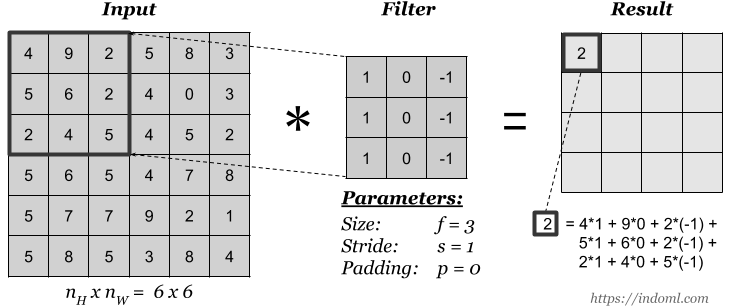
\includegraphics[width=0.85\textwidth, center]{images/convolution-operation.png}
    \caption{Convolution in digital image.}
    \label{fig:conv3}
\end{figure*}

% Jika hasil konvolusi menghasilkan nilai piksel negatif, maka nilai tersebut dijadikan 0, sebaliknya jika hasil konvolusi menghasilkan nilai piksel yang melebihi nilai keabuan maksimum, maka nilai tersebut dijadikan ke nilai keabuan maksimum pada citra tersebut \cite{book:sutoyo}.

If the convolution results in a negative pixel value, then the value is set to 0, on the other hand, if the convolution results in a pixel value that exceeds the maximum gray value, then the value is turned into the maximum gray value of the image \cite{book:sutoyo}.
 

\subsection{Video Stream}
% Video \textit{stream} dapat dipandang sebagai serangkaian citra digital berturut-turut \cite{thesis:jin}. Berbeda dengan format video lainya, video \textit{stream} ini tidak disimpan pada media penyimpanan sebagai file dengan format video melainkan langsung disalurkan setiap framenya dari sumber (\textit{source}) ke penerima, dalam hal ini FPGA.  Dengan menganggap Video \textit{stream} adalah kumpulan citra digital (\textit{frame}) maka dapat dilakukan metode pengolahan seperti pada citra digital, termasuk penerapan filter spasial. 

Video stream can be viewed as a series of consecutive digital images \cite{thesis:jin}. Unlike other video formats, this stream video is not stored on the storage media as a video file format but is directly transmitted each frame from the source to the receiver, in this case the FPGA. By assuming Video stream is a collection of digital images (frame), processing methods such as digital images can be carried out, including the application of spatial filters.


\subsection{FPGA}
% \textit{Field Programmable Gate Arrays} atau FPGA adalah perangkat semikonduktor yang berbasis \textit{matriks configurable logic block} (CLBs) yang terhubung melalui interkoneksi yang dapat diprogram. FPGA dapat diprogram ulang ke aplikasi atau fungsi yang diinginkan setelah \textit{manufacturing}. Fitur ini yang membedakan FPGA dengan \textit{Application Specific Integrated Circuits} (ASICs), yang dibuat khusus untuk tugas tertentu saja \cite{XILINX}.

Field Programmable Gate Arrays or FPGAs are semiconductor devices based on matrix configurable logic blocks (CLBs) connected via programmable interconnects. The FPGA can be reprogrammed to the desired application or function after the manufacturing. This feature is what differentiates FPGAs from the Application Specific Integrated Circuits (ASICs), which are specially made for a specific task \cite{XILINX}.

% Sebuah \textit{microprocessor} menerima instruksi berupa kode 1 atau 0, kode-kode ini selanjutnya diinterpretasikan oleh komputer untuk menjalankan perintah yang diberikan. \textit{Microprocessor} ini membutuhkan intruksi berupa kode secara terus menerus untuk menjalankan fungsinya. Sedangkan pada FPGA hanya dibutuhkan sekali konfigurasi \textit{chip} setiap kali dinyalakan. Membuat atau mengunduh \textit{bitstream} yang menentukan fungsi logika dilakukan oleh \textit{logic elements} (LEs), sebuah sirkuit dapat dibuat dengan mengabungkan beberapa LEs menjadi satu kesatuan. Setelah \textit{bitstream} dipasang, FPGA tidak perlu lagi membaca instruksi berupa 1 dan 0, berbeda dengan \textit{microprocessor} yang selalu membutuhkan instruksi \cite{pdf:cheung}. Secara tradisional, untuk membuat sebuah desain FPGA, aplikasi dideskripsikan menggunakan \textit{Hardware Description Language} (HDL) seperti Verilog atau VHDL sehingga menghasilkan sebuah \textit{bitstream} FPGA.

A microprocessor receives instructions in the form of 1 or 0 code, these codes are then interpreted by the computer to execute the given command. The Microprocessor requires instructions in the form of code continuously to carry out its function. Whereas in FPGA, it only takes to configuration once every time it is powered on. Creating or downloading bitstream which defines logical functions is performed by logic elements (LEs), a circuit can be created by combining multiple LEs into a single unit. After bitstream is installed, the FPGA no longer needs to read instructions in the form of 1 and 0, in contrast to microprocessor which always requires the instruction \cite{pdf:cheung}. Traditionally, to create an FPGA design, applications are described using a Hardware Description Language (HDL) such as Verilog or VHDL so as to produce a bitstream FPGA.


\subsection{FPGA Development Board}

% FPGA \textit{Development Board} atau biasa disebut juga FPGA \textit{Board} yaitu teknologi FPGA yang dirangkai dalam sebuah \textit{board} dan dilengkapi dengan \textit{microprocessor} dan beberapa \textit{interface} \textit{IO} untuk menjalankan tugas tertenu. Umumnya FPGA \textit{Board} telah dilengkapi dengan interface untuk mengakses dan menerapkan desain sirkuitnya. Xilinx, Altera dan Intel adalah produsen FPGA \textit{Board} yang terkenal. FPGA \textit{Board} yang digunakan dalam penelitian ini yaitu Xilinx PYNQ-Z2 dengan Jupyter Notebook sebagai \textit{interface} untuk mengakses dan menjalankan program pada penelitian ini. Bentuk FPGA \textit{Board} Xilinx PYNQ-Z2 dapat dilihat pada gambar (\ref{fig:pynq-z2})

FPGA Development Board or commonly known as FPGA Board, namely FPGA technology that is assembled in a board and is equipped with microprocessor and several interface IO for carry out certain tasks. Generally, FPGA Board is equipped with an interface for accessing and implementing the circuit design. Xilinx, Altera and Intel are well-known FPGA Board manufacturers. The FPGA Board used is the Xilinx PYNQ-Z2 with Jupyter Notebook as the interface to access and run the program in this study. Form of FPGA Board Xilinx PYNQ-Z2 can be seen in figure (\ref{fig:pynq-z2})

\begin{figure}[ht]
    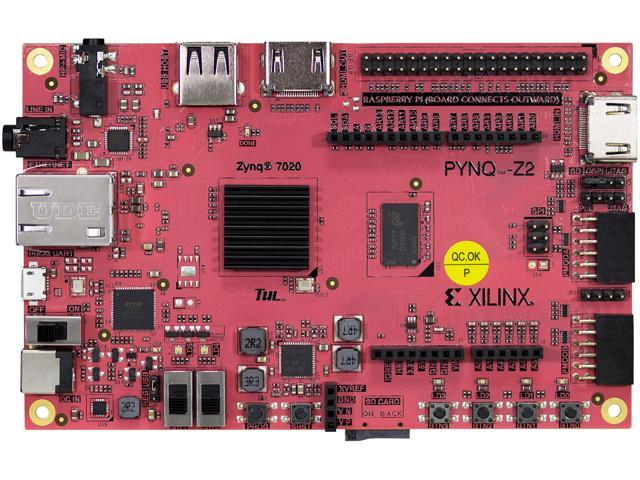
\includegraphics[width=0.8\linewidth, center]{images/pynq-z2.jpeg}
    \caption{FPGA Board Xilinx PYNQ-Z2.}
    \label{fig:pynq-z2}
\end{figure}


\subsection{Performance Evaluatinon}
% Pada penelitian ini peneliti menggunakan waktu komputasi, \textit{frame rate} (FPS), penggunaan CPU, penggunaan {memory}, penggunaan {resident memory} (RES), {shared memory} (SHR), dan {virtual memory} (VIRT) untuk mengukur kinerja pada penerapan filter spasial linear dengan prosesor ARM dan FPGA.

The researchers used computation time, frame rate (FPS), CPU loads, memory usage, resident memory (RES), shared memory (SHR), and virtual memory usage (VIRT) to measure the performance of applying linear spatial filters with ARM and FPGA processors.

\subsubsection{Computation Time}
% Waktu komputasi yang dimaksud oleh peneliti adalah durasi yang dibutuhkan sebuah kernel untuk melakukan filter spasial linear terhadap beberapa \textit{frame} input. Waktu komputasi ini diperoleh dengan cara menghitung selisih waktu selesai dengan waktu dimulai penerapan filter spasial linear pada \textit{frame} input.

The computation time is the duration it takes for a kernel to perform a linear spatial filter on multiple frame inputs. This computation time is obtained by calculating the difference between the finishing time and the starting time of applying linear spatial filters to the input frame.

\begin{equation}
    \label{eq:time}
    \begin{split}
computation\ time = finishing\ time - starting\ time
    \end{split}
\end{equation}

\subsubsection{Frame Rate (FPS)}
% \textit{Frame rate} atau \textit{frame per second} (fps) adalah banyaknya \textit{frame} yang ditampilkan per detik pada video ataupun video \textit{straem}. Semakin tinggi fps sebuah video maka semakin halus pula gerakan yang dihasilkan. Sebaliknya video dengan fps rendah akan menghasilkan gerakan yang kurang baik. \textit{Frame rate} atau fps dapat dihitung dengan cara membagi jumlah \textit{frame} dengan waktu komputasinya seperti pada persamaan \ref{eq:fps} \cite{pdf:pavan}.

Frame rate or frames per second (fps) is the number of frames displayed per second on a video or video straem. The higher the fps of a video, the smoother the result. On the other hand, videos with low fps will result in poor motion. Frame rate or fps can be calculated by dividing the number of frames by the computation time as in the equation \ref{eq:fps} \cite{pdf:pavan}.

\begin{equation}
    \label{eq:fps}
    \begin{split}
fps = \frac{number\ of\ frame}{computation\ time}
    \end{split}
\end{equation}

\subsubsection{CPU Loads}
% Pada penelitian ini peneliti menggunakan fitur yang tersedia pada sistem operasi Linux yang berjalan di FPGA Development Board untuk melihat persentase penggunaan CPU pada proses penerapan filter spasial linear. Program ini menampilkan informasi tentang proses-proses yang berjalan pada sistem operasi seperti ID sebuah proses, user yang menjalankan proses tersebut, \textit{memory} yang digunakan, status sebuah proses, persentase CPU yang digunakan dan lainnya.

The researchers used the features available on the Linux operating system running on the FPGA Development Board to see the percentage of CPU loads in the process of applying linear spatial filters. This program displays information about processes running on the operating system such as the ID of a process, the user running the process, the memory used, the status of a process, the percentage of CPU used and others.

\subsubsection{Memory Utilize}

% Pada sistem operasi linux \textit{memory} dibagi menjadi tiga jenis \cite{manual:linux}. Pertama yaitu \textit{memory} fisik, sumber daya terbatas di mana kode dan data harus berada saat dijalankan atau direferensikan. Berikutnya adalah \textit{memory} \textit{swap}, yaitu  \textit{memory} yang berguna untuk membantu kerja \textit{memory} fisik, data dari \textit{memory} fisik akan disimpan pada \textit{swap} dan kemudian diambil kembali jika terlalu banyak permintaan pada \textit{memory} fisik. Ketiga yaitu virtual \textit{memory}, sumber daya yang hampir tidak terbatas yang digunakan untuk tujuan berikut \cite{book:os}:

On the linux operating system memory is divided into three types \cite{manual:linux}. The first is the physical memory, a finite resource that code and data must reside in when executed or referenced. Next is memory swap, which is memory that useful for helping physical memory work, data from physical memory will be stored in swap and then retrieved return if too many requests to physical memory. The third is virtual memory, an almost unlimited resource used for the following purposes \cite{book:os}:

\begin{itemize} [noitemsep, topsep=0pt]
    \item \textit{abstraction}, free of physical memory addresses / boundaries
    \item \textit{isolation}, each process in a separate address space 
    \item \textit{sharing}, a single map can meet many needs 
    \item \textit{flexibility}, assign virtual addresses to data
\end{itemize}

\subsubsection{Virtual Memory (VIRT)}
% Virtual \textit{memory} menggunakan disk sebagai perpanjangan dari RAM sehingga ukuran efektif \textit{memory} yang dapat digunakan bertambah secara bersamaan. Kernel akan menulis konten dari blok \textit{memory} yang saat ini tidak digunakan ke hard disk sehingga \textit{memory} dapat digunakan untuk tujuan lain. Ketika konten asli dibutuhkan lagi, mereka dibaca kembali ke dalam \textit{memory}. Ini semua dibuat transparan sepenuhnya bagi pengguna. Program yang berjalan di Linux hanya melihat jumlah \textit{memory} yang tersedia lebih besar dan tidak memperhatikan bahwa sebagian dari program tersebut berada di disk dari waktu ke waktu. Tentu saja, membaca dan menulis hard disk lebih lambat daripada menggunakan \textit{memory} fisik, sehingga program tidak berjalan secepat itu. Bagian dari hard disk yang digunakan sebagai \textit{memory} virtual disebut ruang swap \cite{site:ltdp}.

Virtual memory uses disk as an extension of RAM so that the effective size of the usable memory increases simultaneously. The kernel will write the contents of the currently unused memory block to the hard disk so that memory can be used for other purposes. When the original content is needed again, they are read back into memory. These are all made completely transparent to the user. Programs running on Linux only see the larger amount of memory available and do not notice that some of them are on disk over time. Of course, reading and writing a hard disk is slower than using physical memory, so programs don't run that fast. The part of the hard disk that is used as virtual memory is called swap space \cite{site:ltdp}.

\subsubsection{Resident Memory (RES)}

% \textit{Resident} \textit{memory} adalah bagian dari ruang alamat virtual (VIRT) yang mewakili \textit{memory} fisik yang tidak ditukar yang sedang digunakan tugas. Resident \textit{memory} ini juga merupakan penjumlahan dari RSan, RSfd dan Bidang RSsh. Ini dapat mencakup private anonymous \textit{pages}, halaman pribadi yang dipetakan ke file (termasuk \textit{program images} dan \textit{shared libraries}) ditambah shared anonymous \textit{pages}. Semua \textit{memory} tersebut didukung oleh file \textit{swap} yang direpresentasikan secara terpisah pada SWAP. Resident \textit{memory} ini juga dapat menyertakan \textit{pages} yang didukung \textit{shared file-backed} yang apabila dimodifikasi, maka akan bertindak sebagai file \textit{swap} khusus dan karenanya tidak akan pernah memengaruhi SWAP \cite{manual:linux}.

Resident memory is the portion of the virtual address space (VIRT) that represents the unchanged physical memory that the task is currently running. Resident memory is also the sum of the RSan, RSfd and RSsh fields. This can include private anonymous pages, private pages mapped to files (including program images and shared libraries) plus shared anonymous pages. All such memory is supported by a swap file which is represented separately on SWAP. This resident memory can also include a supported pages shared file-backed which, when modified, acts as a custom swap file and therefore never affects SWAP \cite{manual:linux}.

\subsubsection{Shared Memory (SHR)}

% \textit{Shared} \textit{memory} adalah bagian dari resident \textit{memory} (RES) yang dapat digunakan oleh proses lain. Termasuk \textit{anonymous pages} dan shared file-backed \textit{pages}. Ini juga termasuk private \textit{pages} dipetakan ke file yang mewakili \textit{program images} dan \textit{shared libraries} \cite{manual:linux}. 

Shared memory is a part of resident memory (RES) that can be used by other processes. Includes anonymous pages and shared file-backed pages. This also includes private pages mapped to files representing program images and shared libraries \cite{manual:linux}.


%------------------------------------------------
% 3. Tools and Methods

\section{Tools and Methods}

\subsection{System Design}
\begin{figure}[ht]
    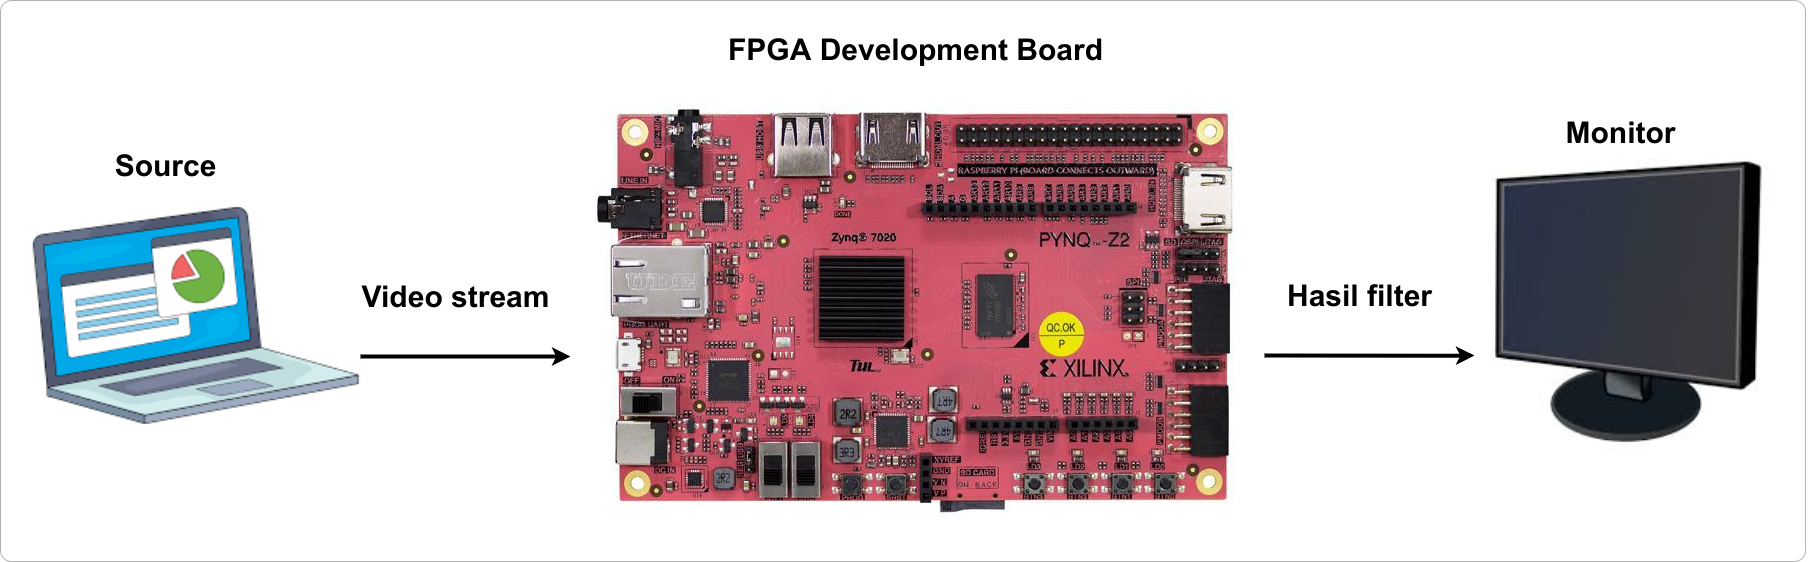
\includegraphics[width=1\linewidth, center]{images/rancangan-sistem2.png}
    \caption{System Design.}
    \label{fig:rancangan-sistem}
\end{figure}

% Video \textit{stream} dari \textit{source} disalurkan melalui port HDMI Input pada FPGA Development Board, kemudian video \textit{stream} tersebut akan diolah dengan menerapkan filter spasial linear pada setiap framenya. Setiap \textit{frame} yang telah diterapkan filter spasial akan dialirkan ke monitor untuk kemudian ditampilkan. Selanjutnya dilakukan analisis kinerja pada FPGA. FPGA Development Board yang digunakan dalam penelitian ini dapat diakses dengan \textit{ssh} pada port 22 atau dengan \textit{Jupyter Notebook} melalui \textit{web browser}.

Video stream from the source is channeled through the HDMI Input port on the FPGA Development Board, then the video stream will be processed by applying a linear spatial filter to each frame. Each frame that has been applied the spatial filter will be streamed to the monitor to display. Furthermore, the FPGA performance analysis is carried out. The FPGA Development Board used can be accessed with ssh protocol on port 22 or by Jupyter Notebook via web browser.

\subsection{Tools}
\begin{enumerate}[topsep=0pt,itemsep=0pt,partopsep=0pt, parsep=0pt]
    \item Software requirements:
    \begin{enumerate}[topsep=0pt,itemsep=0pt,partopsep=0pt, parsep=0pt, label={\alph*.}]
        \item Linux Ubuntu 18, Operation sistem on FPGA Development Board.
        \item Python 3.6, library OpenCV, Numpy, Pynq 5.2, and Xilinx xfOpenCV.
        \item Jupyter Notebook on FPGA Development Board. 
        \item Web Browser.
    \end{enumerate}
    \item Hardware requirements:
    \begin{enumerate}[topsep=0pt,itemsep=0pt,partopsep=0pt, parsep=0pt, label={\alph*.}]
        \item FPGA Development Board.
        \item Micro SD Card 16 GB.
        \item Eksternal Monitor, to display the results of applying spatial filters on the FPGA Development Board.
        \item Lenovo Ideapad 320 as \textit{source} of video stream).
    \end{enumerate}

    FPGA Development Board specification:
    \begin{itemize}[topsep=0pt,itemsep=0pt,partopsep=0pt, parsep=0pt]
        \item Model : Xilinx PYNQ-Z2.
        \item Processor : Dual-Core ARM Cortex A9, 650 MHz
        \item FPGA : 1,3M reconfigurable gates
        \item Memory : 512 MB DDR3 / Flash
        \item Storage : Micro SD card slot
        \item Power : DC 7V-15V
        \item Dimension : 3,44" x 5,39" (87mm x 137mm)
    \end{itemize}
\end{enumerate}


\subsection{Methods}

% Proses filter spasial dilakukan dengan operasi konvolusi pada setiap matriks dengan kernel yang telah ditentukan sebelumnya. Operasi konvolusi ini menghasilkan matrix baru dengan ukuran 1280x720. Matriks hasil tersebut selanjutnya direpresentasikan kembali sebagai citra digital yang selanjutnya disebut sebagai hasil filter. Hasil filter dari setiap \textit{frame} ini ditampilkan ke monitor melalui HDMI Output pada FPGA Development Board secara berkesinambungan sehingga tampak seperti video.

The spatial filter process is carried out by convolution operations on each matrix with a predetermined kernel. This convolutional operation produces a new matrix 1280x720. The resulting matrix is then represented as a digital image, hereinafter referred to as the filter result. The filter result of each frame is displayed to the monitor via HDMI Output on the FPGA Development Board continuously.

\begin{figure}[H]
    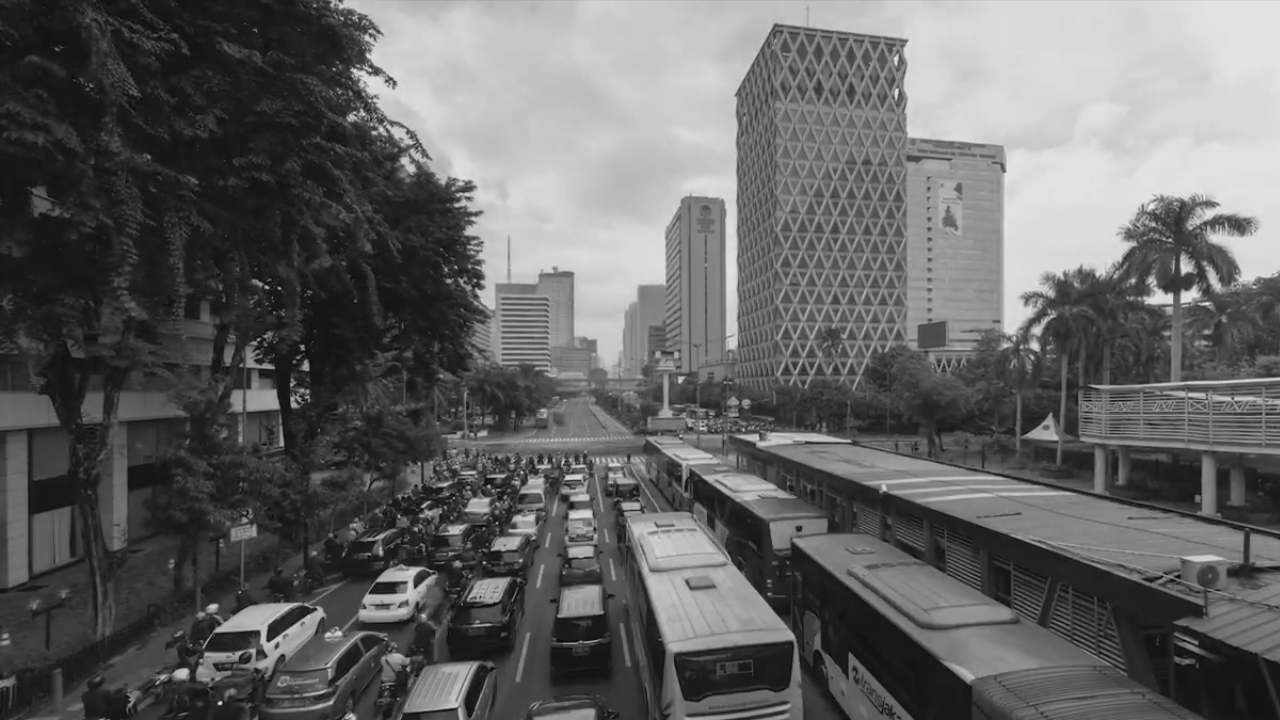
\includegraphics[width=0.8\linewidth, center]{images/output-image/input1-grayscale.png}
    \caption{Grayscale Frame.}
    \label{fig:input-grayscale}
\end{figure}


\subsubsection{Average Blur}
% Penerapan filter spasial pada \textit{frame} \textit{grayscale} yang berukuran 1280x720 pixel dengan kernel \textit{average blur} (\ref{kernel:average}) yang berukuran 3x3 menghasilkan citra \textit{blur} yang berukuran 1280x720. Hasil filter \textit{average blur} dapat dilihat pada gambar \ref{fig:output-averageblur}. Filter seperti ini dapat digunakan untuk mengurangi derau pada citra.

Applying a spatial filter to grayscale frame which is 1280x720 pixels using a kernel average blur  (\ref{kernel:average}) measuring 3x3 produces a blur image that is 1280x720 too. The results of the average blur filter can be seen in the \ref{fig:output-averageblur} image. Filters like this can be used to reduce noise in the image.

\begin{figure}
    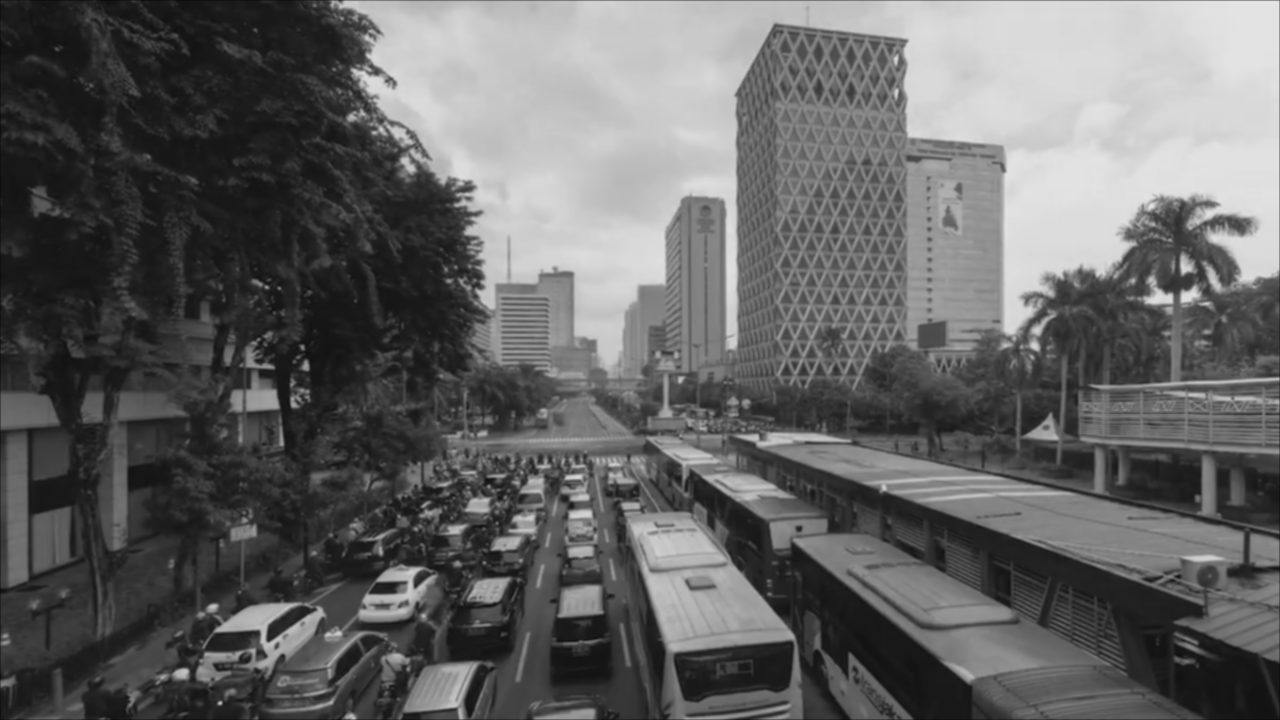
\includegraphics[width=0.8\linewidth, center]{images/output-image/input1-averageblur.png}
    \caption{Result of Average Blur filter.}
    \label{fig:output-averageblur}
\end{figure}

\subsubsection{Gaussian Blur}
% Penerapan filter spasial dengan kernel \textit{gaussian blur} (\ref{kernel:gaussianblur}) yang berukuran 3x3 menghasilkan citra \textit{blur} yang secara kasat mata mirip dengan filter \textit{average blur}. Namun apabila diperhatikan nilai masing-masing pixel pada gambar \ref{fig:output-gaussianblur} akan terlihat berbeda dengan nilai masing-masing pixel pada gambar \ref{fig:output-averageblur}. Hal ini disebabkan oleh nilai bobot pada kernel \textit{gaussian blur} yang berbeda dengan kernel \textit{average blur} sehingga hasil konvolusinya juga berbeda. 

The application of a spatial filter with a 3x3 kernel gaussian blur (\ref{kernel:gaussianblur}) produces a blur image which is visually similar to the average blur filter. However, if you pay attention to the value of each pixel in the figure \ref{fig:output-gaussianblur} it will look different from the value of each pixel in the figure \ref{fig:output-averageblur}. This is because the weight value in the gaussian blur kernel is different from the average blur kernel, so the result of the convolution is also different.

\begin{figure}
    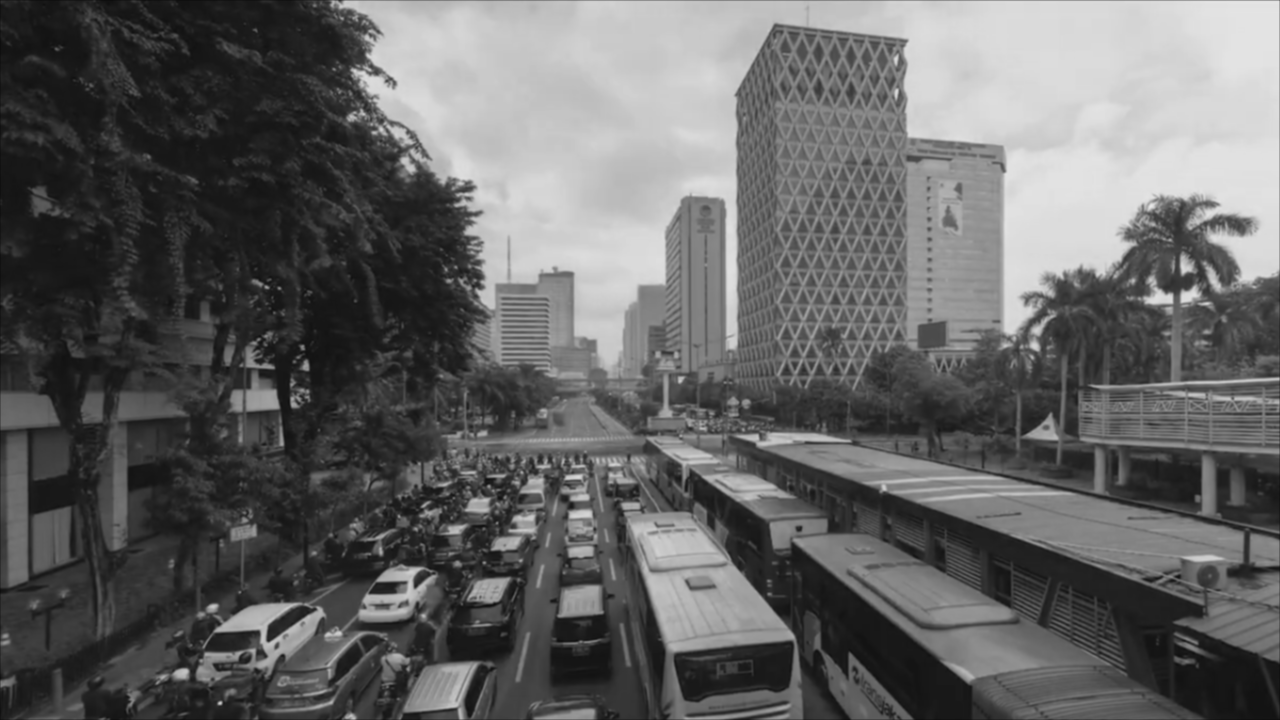
\includegraphics[width=0.8\linewidth, center]{images/output-image/input1-gaussianblur.png}
    \caption{Result of Gaussian Blur filter.}
    \label{fig:output-gaussianblur}
\end{figure}

\subsubsection{Laplacian}
% Penerapan filter spasial dengan kernel \textit{laplacian} (\ref{kernel:laplacian}) menghasilkan citra \textit{biner} yang hanya direpresentasikan dengan warna hitam dan putih saja, dapat dilihat pada gambar \ref{fig:output-laplacian}. Filter seperti ini dapat digunakan pada metode deteksi tepi dalam proses pengolahan citra digital.

Application of spatial filter with kernel laplacian (\ref{kernel:laplacian}) produces binary image which is represented only in black and white, can be seen in figure \ref{fig:output-laplacian}. Filters like this can be used in edge detection methods in digital image processing.

\begin{figure}
    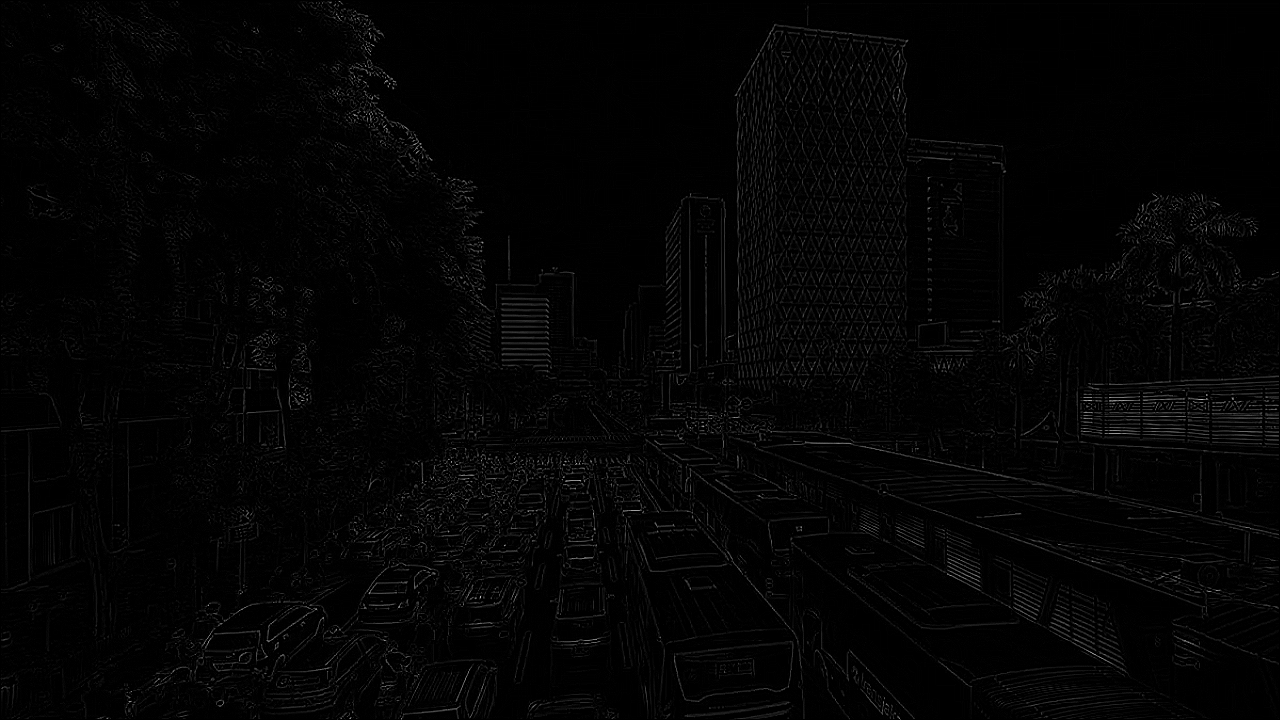
\includegraphics[width=0.8\linewidth, center]{images/output-image/input1-laplacian.png}
    \caption{Result of Laplacian filter.}
    \label{fig:output-laplacian}
\end{figure}

\subsubsection{Sharpening}
% Penerapan filter spasial dengan kernel \textit{sharpening} (\ref{kernel:sharpen}) dapat meningkatkan detail (seperti garis) pada citra, namun dapat juga dapat menimbulkan derau pada citra apabila bobot kernelnya tidak sesuai. Filter seperti ini lebih tepat digunakan untuk memperbaiki kualitas citra (dengan nilai kernel yang sesuai). Hasil filter \textit{sharpening} ini dapat dilihat pada gambar \ref{fig:output-sharpen}.

Applying a spatial filter with kernel sharpening (\ref{kernel:sharpen}) can increase detail (such as lines) in the image, but can also cause noise in the image if the kernel weight is not appropriate. Filters like this are more appropriate to improve image quality (with the appropriate kernel values). The results of the sharpening filter can be seen in the \ref{fig:output-sharpen} image.

\begin{figure}
    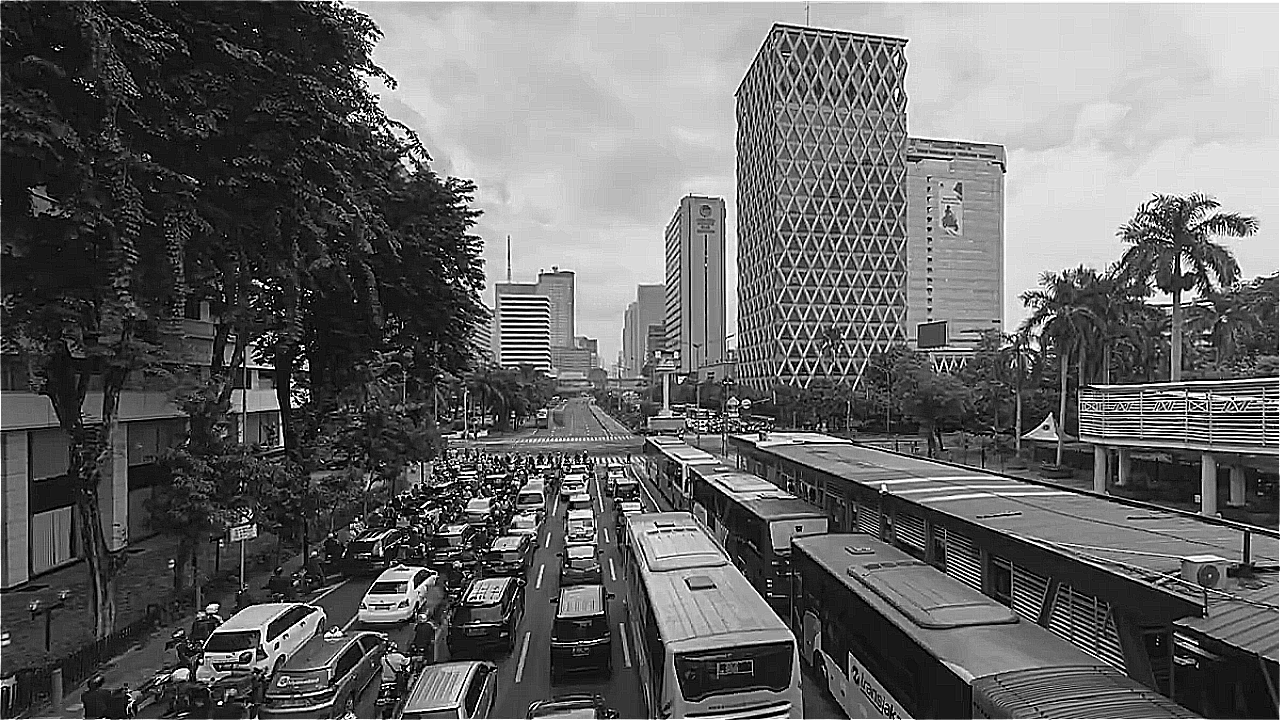
\includegraphics[width=0.8\linewidth, center]{images/output-image/input1-sharpen.png}
    \caption{Result of Sharpening filter.}
    \label{fig:output-sharpen}
\end{figure}

\subsubsection{Sobel Horizontal}
% Penerapan filter spasial dengan kernel \textit{sobel horizontal} (\ref{kernel:sobel}) menghasilkan citra \textit{biner}, dapat dilihat pada gambar \ref{fig:output-sobelhor}. Filter seperti lebih tepat digunakan pada metode deteksi tepi dengan citra yang banyak mengandung garis horizontal.

Application of a spatial filter with kernel sobel horizontal (\ref{kernel:sobel}) produces a binary image, seen in figure \ref{fig:output-sobelhor}. Such filters are more appropriate for edge detection methods with images that contain lots of horizontal lines.

\begin{figure}
    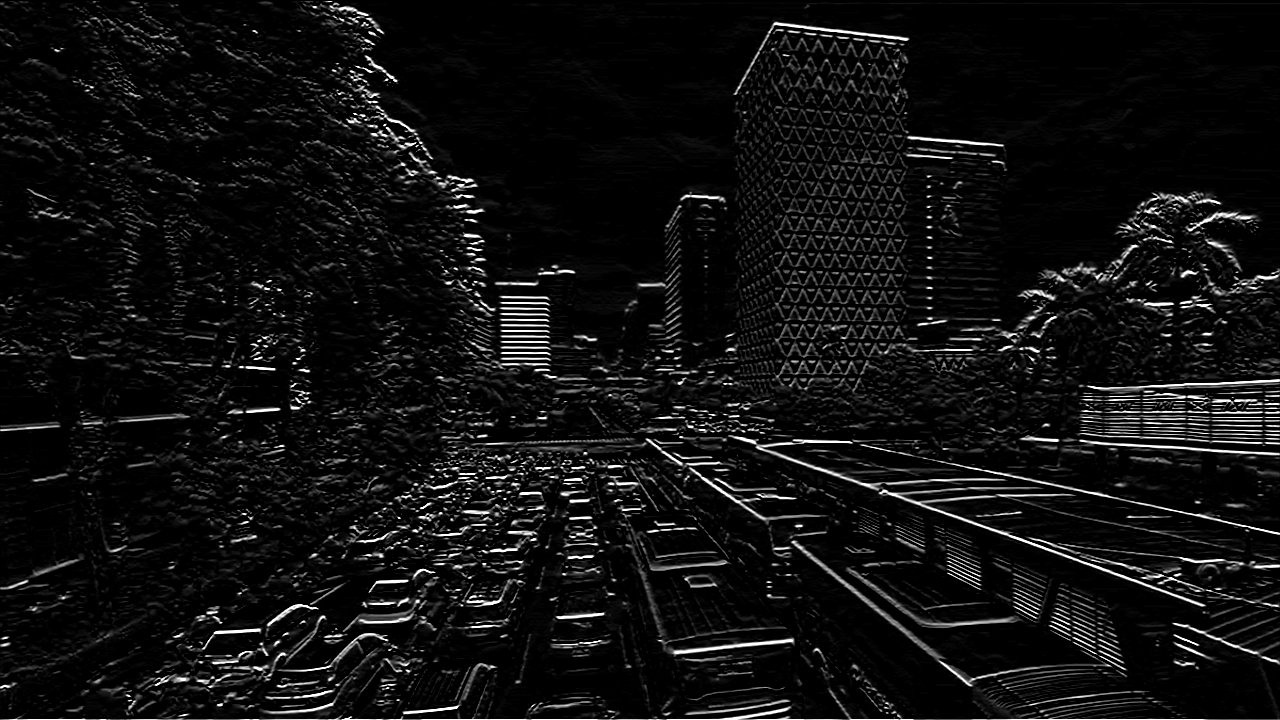
\includegraphics[width=0.8\linewidth, center]{images/output-image/input1-sobelhor.png}
    \caption{Result of Sobel Horizontal filter.}
    \label{fig:output-sobelhor}
\end{figure}

\subsubsection{Sobel Vertical}
% Penerapan filter spasial dengan kernel \textit{sobel vertical} (\ref{kernel:sobel}) menghasilkan citra \textit{biner}, dapat dilihat pada gambar \ref{fig:output-sobelver}. Sama halnya dengan filter \textit{sobel horizontal}, filter \textit{sobel vertical} juga dapat digunakan untuk metode deteksi tepi, terutama pada citra yang banyak mengandung garis vertikal.

Application of a spatial filter with kernel sobel vertical (\ref{kernel:sobel}) produces a binary image, seen in figure \ref{fig:output-sobelver}. Similar to the sobel horizontal filter, the sobel vertical filter can also be used for edge detection methods, especially on images that contain lots of vertical lines.

\begin{figure}
    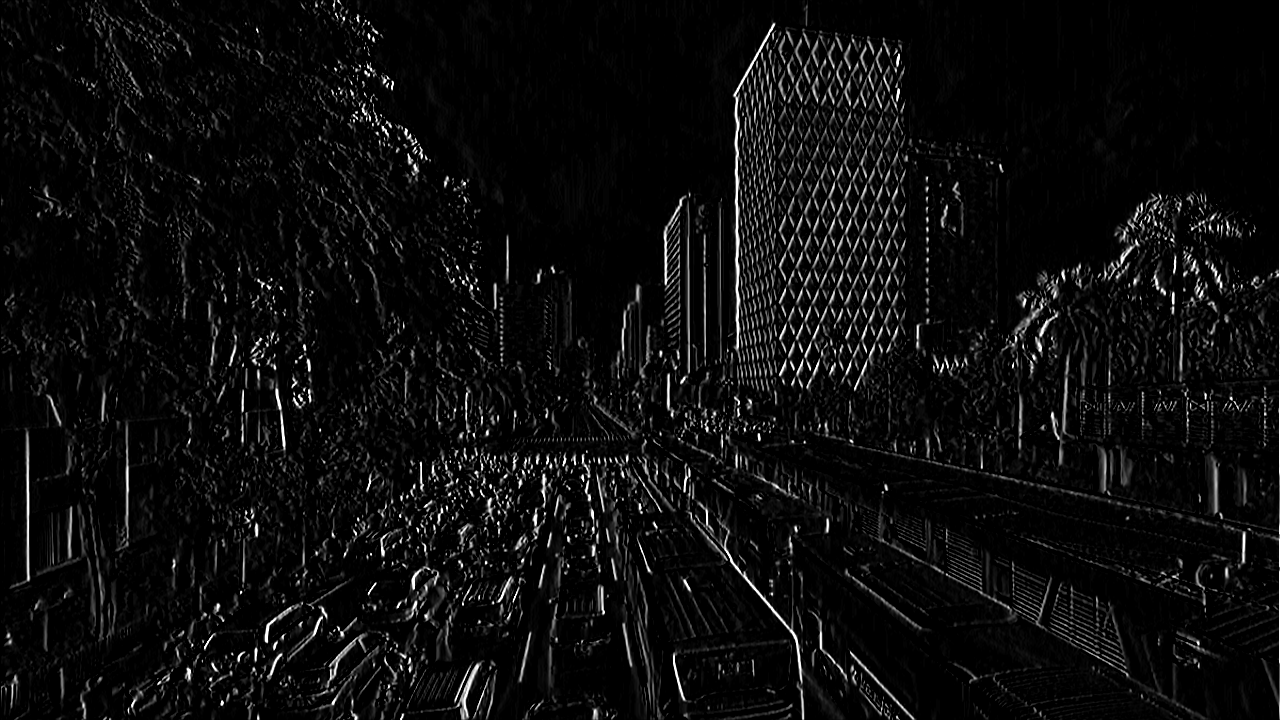
\includegraphics[width=0.8\linewidth, center]{images/output-image/input1-sobelver.png}
    \caption{Result of Sobel Vertical filter.}
    \label{fig:output-sobelver}
\end{figure}


%------------------------------------------------
% 4. Results and Discussions

\section{Results and Discussions}

\subsection{Computation Time}

% Data waktu komputasi dengan menggunakan 50 frame pada masing-masing kernel dapat dilihat pada tabel \ref{table:hasil-time50} dan grafik pada gambar \ref{fig:chart-time50}. Secara umum waktu komputasi dengan menggunakan prosesor ARM lebih lambat daripada waktu komputasi dengan menggunakan FPGA. Rata-rata waktu komputasi dengan prosesor ARM menggunakan 50 frame adalah 7,26 detik, sedangkan rata-rata waktu komputasi dengan FPGA menggunakan 50 frame hanya 0,82 detik.

The computation time using 50 frames in each kernel can be seen in the \ref{table:result-time50} table and the chart in figure \ref{fig:chart-time50}. In general, the computation time using an ARM processor is slower than FPGA. The average computation time with an ARM processor using 50 frames was 7.26 seconds, while the average computation time with an FPGA using 50 frames was only 0.82 seconds.

\begin{atable}
    \caption{Comparison table of Computing time using 50 frames.}
    \label{table:hasil-time50}
    \csvreader[
        head to column names,
        tabular=lcc,
        separator=semicolon,
        before table=\rowcolors{2}{gray!15}{gray!30},
        table head= \rowcolor{gray!50!black} 
            \color{white} Filter & 
            \color{white} Prosesor ARM (s) & 
            \color{white} FPGA (s)\\]
        {tables/hasil-time50.csv}
        {
            filter=\filter, 
            arm=\arm, 
            fpga=\fpga}
        {
            \filter & 
            \arm & 
            \fpga }
\end{atable}
\begin{figure}[ht]
    \centering
    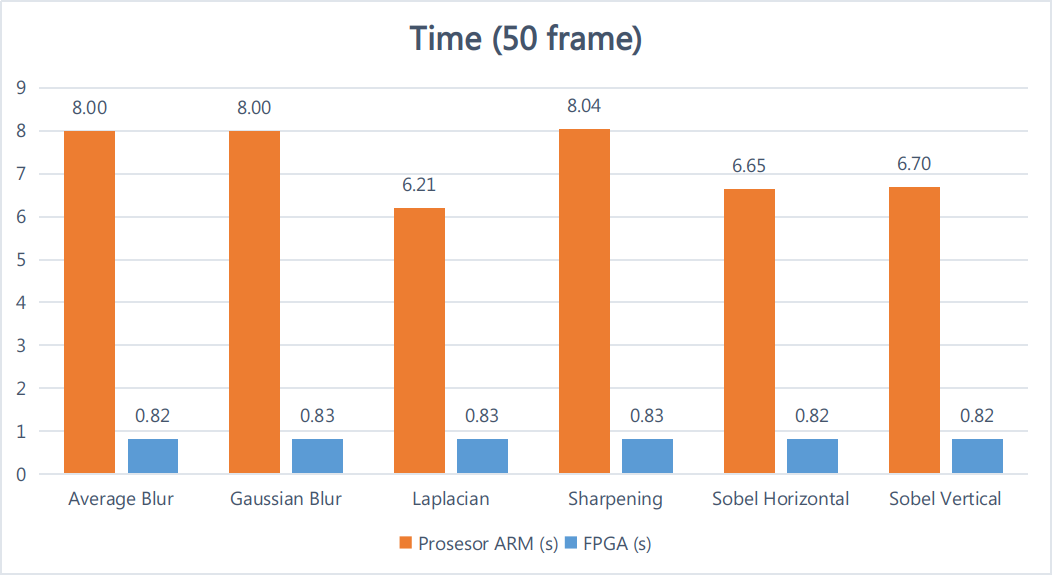
\includegraphics[width=0.81\linewidth, center]{images/chart/chart-time50.png}
    \caption{Comparison chart of Computing time using 50 frames}
    \label{fig:chart-time50}
\end{figure}

% Data waktu komputasi menggunakan 200 frame pada maasing-masing kernel dapat dilihat pada tabel \ref{table:hasil-time200} dan grafik pada gambar \ref{fig:chart-time200}. Rata-rata waktu komputasi dengan prosesor ARM menggunakan 200 frame adalah 29,06 detik, sedangkan rata-rata waktu komputasi dengan FPGA menggunakan 200 frame hanya 3,32 detik.

The computation time data using 200 frames in each kernel can be seen in the table \ref{table: result-time200} and the chart in figure \ref{fig:chart-time200}. The average computation time with an ARM processor using 200 frames was 29.06 seconds, while the average computation time with an FPGA using 200 frames was only 3.32 seconds.

\begin{atable}
    \caption{Comparison table of Computing time using 200 frames.}
    \label{table:hasil-time200}
    \csvreader[
        head to column names,
        tabular=lcc,
        separator=semicolon,
        before table=\rowcolors{2}{gray!15}{gray!30},
        table head= \rowcolor{gray!50!black} 
            \color{white} Filter & 
            \color{white} Prosesor ARM (s) & 
            \color{white} FPGA (s)\\]
        {tables/hasil-time200.csv}
        {
            filter=\filter, 
            arm=\arm, 
            fpga=\fpga}
        {
            \filter & 
            \arm & 
            \fpga }
\end{atable}

\begin{figure}[ht]
    \centering
    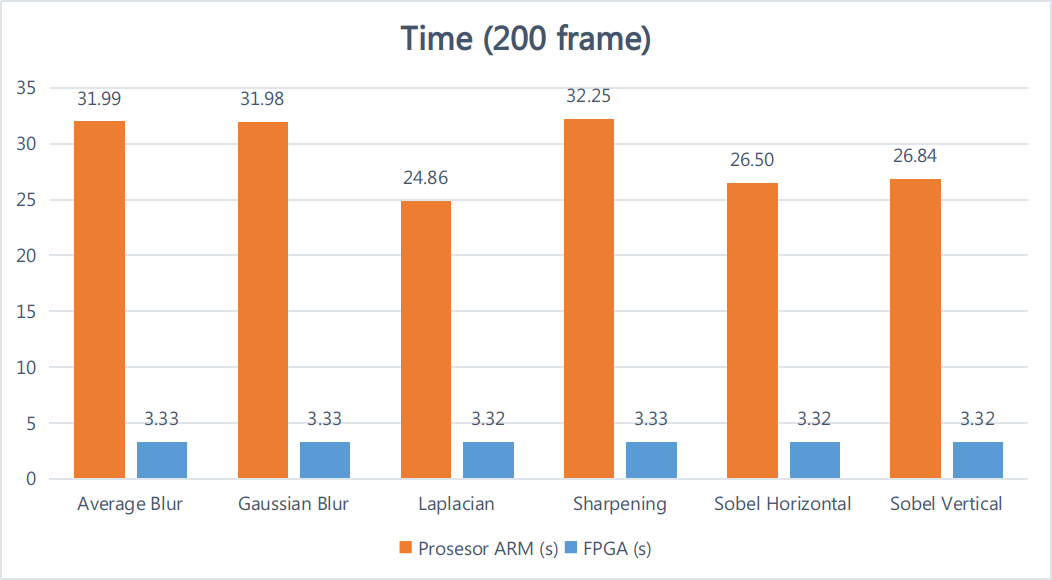
\includegraphics[width=0.81\linewidth, center]{images/chart/chart-time200.png}
    \caption{Comparison chart of Computing time using 200 frames.}
    \label{fig:chart-time200}
\end{figure}

% Waktu komputasi tercepat dengan menggunakan prosesor ARM terdapat pada filter \textit{laplacian} yaitu 6,21 detik dengan 50 frame dan 24.85 detik dengan 200 frame. Sedangkan waktu komputasi paling lambat ketika menggunakan prosesor ARM terdapat pada filter \textit{sharpening} yaitu 8,04 detik dengan 50 frame dan 32,24 detik dengan 200 frame. 

The fastest computation time using an ARM processor is the laplacian filter, namely 6.21 seconds with 50 frames and 24.85 seconds with 200 frames. Meanwhile, the slowest computation time when using an ARM processor is the sharpening filter, namely 8.04 seconds with 50 frames and 32.24 seconds with 200 frames.

% Untuk menghitung efisiensi waktu komputasi yang dimiliki FPGA dibandingkan dengan prosesor ARM, digunakan rumus:

To calculate the computation time efficiency of an FPGA compared to an ARM processor, the formula is used:
\begin{equation*}
    % \label{eq:efisiensi}
    \begin{split}
& = 100\% - \left( \frac{computation\ time\ FPGA}{computation\ time\ ARM Prosesor} \times 100\% \right) \\
& = 100\% - \left( \frac{3,32}{29,06} \times 100\% \right) \\
& = 100\% - 11.42\% \\
& = 88.58\% \\
    \end{split}
\end{equation*}
% sehingga diperoleh efisiensi waktu komputasi FPGA dibandingkan dengan prosesor ARM adalah sebesar 88.85\%.

the efficiency of FPGA computation time compared to ARM processors is 88.85\%.

\subsection{Frame Rate (FPS)}
% Dengan mengetahui waktu komputasi dan jumlah frame maka frame rate atau FPS dapat dihitung menggunakan persamaan \ref{eq:fps}. Data FPS dari masing-masing kernel dengan prosesor ARM dan FPGA dapat dilihat pada tabel \ref{table:hasil-fps} dan grafik pada gambar \ref{fig:chart-fps}.

By the computation time and the number of frames, the frame rate or FPS can be calculated using the \ref{eq:fps} equation. FPS data for each kernel with ARM and FPGA processors can be seen in the \ref{table:fps-result} table and the chart in the figure \ref{fig:chart-fps}.
\begin{atable}
    \caption{Comparison table of FPS using ARM prosesor and FPGA.}
    \label{table:hasil-fps}
    \csvreader[
        head to column names,
        tabular=lcc,
        separator=semicolon,
        before table=\rowcolors{2}{gray!15}{gray!30},
        table head= \rowcolor{gray!50!black} 
            \color{white} Filter & 
            \color{white} Prosesor ARM & 
            \color{white} FPGA\\]
        {tables/hasil-fps.csv}
        {
            filter=\filter, 
            arm=\arm, 
            fpga=\fpga}
        {
            \filter & 
            \arm & 
            \fpga }
\end{atable}
\begin{figure}[H]
    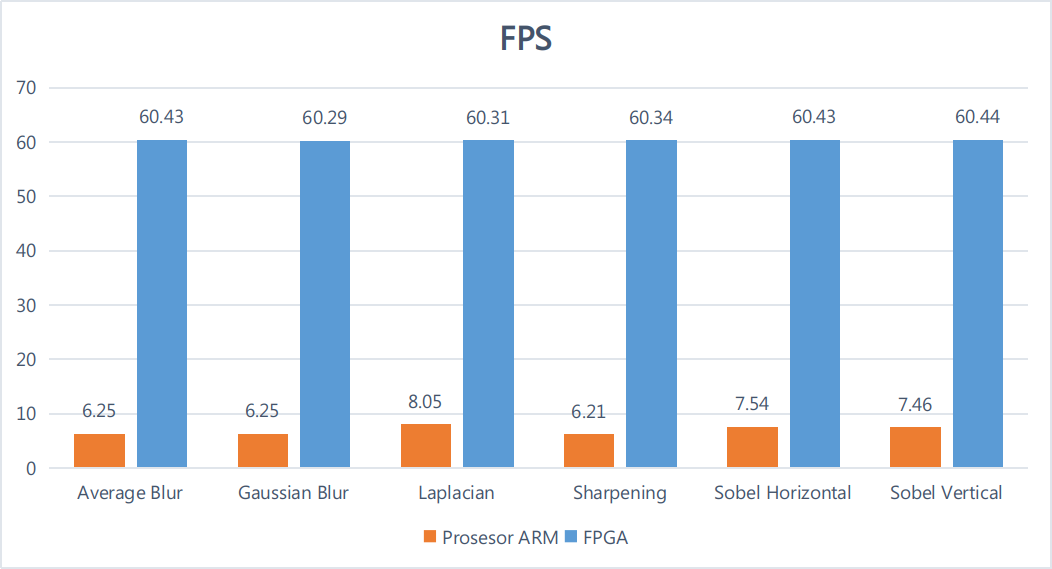
\includegraphics[width=0.81\linewidth, center]{images/chart/chart-fps.png}
    \caption{Comparison chart of FPS using ARM prosesor and FPGA.}
    \label{fig:chart-fps}
\end{figure}

% Pada tabel \ref{table:hasil-fps} terlihat dengan menggunakan prosesor ARM diperoleh rata-rata 6.95 frame per detik (FPS), sedangkan ketika menggunakan FPGA diperoleh rata-rata 60.37 frame per detik. Terlihat pada grafik \ref{fig:chart-fps} nilai FPS dengan FPGA jauh lebih tinggi daripada dengan prosesor ARM.

In the table \ref{table:hasil-fps}, it can be seen that using an ARM processor the average is 6.95 frames per second (FPS) was obtained, while using an FPGA the average is 60.37 frames per second was obtained. As seen in the chart \ref{fig:chart-fps} the FPS value with FPGA is much higher than with an ARM processor.

% Untuk menghitung efisiensi FPS yang dimiliki FPGA dibandingkan dengan prosesor ARM, digunakan rumus:

To calculate the FPS efficiency that the FPGA has compared to an ARM processor, the formula is used:
\begin{equation*}
    % \label{eq:efisiensi}
    \begin{split}
& = 100\% - \left( \frac{FPS\ ARM Prosesor}{FPS\ FPGA} \times 100\% \right) \\
& = 100\% - \left( \frac{6.95}{60.37} \times 100\% \right) \\
& = 100\% - 11.51\% \\
& = 88.49\% \\
    \end{split}
\end{equation*}

% sehingga diperoleh efisiensi FPS dari FPGA dibandingkan dengan prosesor ARM adalah sebesar 88.49\%.

the FPS efficiency of the FPGA compared to the ARM processor is 88.49\%.

\subsection{CPU Loads}

% Data perbandingan penggunaan CPU pada masing-masing kernel dengan prosesor ARM dan FPGA dapat dilihat pada tabel \ref{table:hasil-cpu} dan grafik pada gambar \ref{fig:chart-cpu}. Rata-rata penggunaan CPU dengan prosesor ARM adalah 99.58\% sedangkan dengan FPGA diperoleh 84.75\%. Data ini menunjukkan bahwa penggunaan CPU dengan prosesor ARM sedikit lebih besar daripada dengan FPGA.

Comparative data on CPU loads on each kernel with ARM and FPGA processors can be seen in the \ref{table:cpu-result} table and the chart in the \ref{fig:chart-cpu} table. The average CPU loads with ARM processors is 99.58\% while with FPGA it is 84.75\%. This data shows that CPU loads with ARM processors is slightly greater than with FPGAs.

\begin{atable}
    \caption{Comparison table of cpu usage using ARM prosesor and FPGA.}
    \label{table:hasil-cpu}
    \csvreader[
        head to column names,
        tabular=lcc,
        separator=semicolon,
        before table=\rowcolors{2}{gray!15}{gray!30},
        table head= \rowcolor{gray!50!black} 
            \color{white} Filter & 
            \color{white} Prosesor ARM (\%) & 
            \color{white} FPGA (\%)\\]
        {tables/hasil-cpu.csv}
        {
            filter=\filter, 
            arm=\arm, 
            fpga=\fpga}
        {
            \filter & 
            \arm & 
            \fpga }
\end{atable}
\begin{figure}[H]
    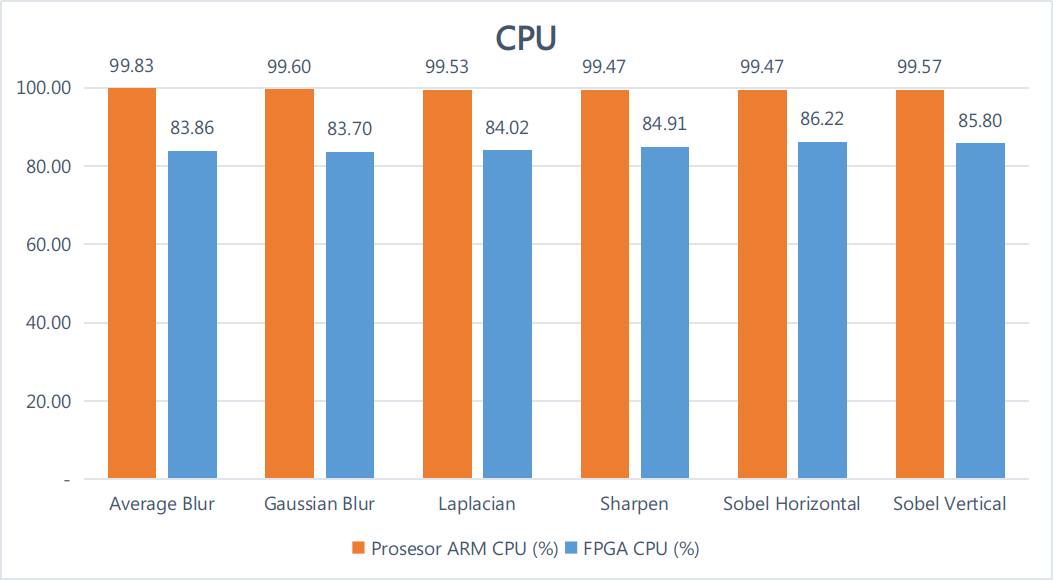
\includegraphics[width=0.81\linewidth, center]{images/chart/chart-cpu.png}
    \caption{Comparison chart of CPU loads using ARM prosesor and FPGA.}
    \label{fig:chart-cpu}
\end{figure}

% Penggunaan CPU terbesar dengan prosesor ARM yaitu pada kernel \textit{average blur} (99,83\%) dan dengan FPGA pada kernel \textit{sobel horizontal} (86,22\%). Penggunaan CPU terkecil dengan prosesor ARM yaitu pada kernel \textit{sharpening} dan \textit{sobel horizontal} (99,47\%) dan dengan FPGA pada kernel \textit{gaussian blur} (83,70\%).

The biggest CPU loads with ARM processors is the average blur kernel (99.83\%) and the FPGA on the sobel horizontal kernel (86.22\%). The CPU loads with ARM processors is the sharpening and sobel horizontal kernel (99.47\%) and with the FPGA on the gaussian blur kernel (83.70\%).

% Untuk menghitung efisiensi penggunaan CPU yang dimiliki FPGA dibandingkan dengan prosesor ARM, digunakan persamaan berikut:

To calculate the CPU loads efficiency of an FPGA compared to an ARM processor, the following equation is used:
\begin{equation*}
    % \label{eq:efisiensi}
    \begin{split}
& = 100\% - \left( \frac{CPU\ FPGA}{CPU\ ARM Prosesor} \times 100\% \right) \\
& = 100\% - \left( \frac{84.75}{99.58} \times 100\% \right) \\
& = 100\% - 85.11\% \\
& = 14.89\% \\
    \end{split}
\end{equation*}
% sehingga diperoleh efisiensi penggunaan CPU FPGA dibandingkan dengan prosesor ARM adalah sebesar 14.89\%.

the efficiency of FPGA CPU loads compared to ARM processors is 14.89\%.


\subsection{Memory Utilize}

% Data penggunaan \textit{memory} dengan prosesor ARM dan FPGA dapat dilihat pada tabel \ref{table:hasil-mem} dan grafik pada gambar \ref{fig:chart-mem}. Data ini menunjukkan persentase \textit{memory} yang digunakan pada masing-masing kernel. Rata-rata penggunaan \textit{memory} dengan prosesor ARM adalah 25,37\% dan 24,86\% dengan FPGA. 

Memory utilize with ARM processors and FPGA can be seen in the \ ref{table:mem-results} table and the chart in the \ref{fig:chart-mem} image. This data shows the percentage memory used in each kernel. The average usage of memory with an ARM processor is 25.37\% and 24.86\% with an FPGA.

\begin{atable}
    \caption{Comparison table of Memory Utilize using ARM prosesor and FPGA.}
    \label{table:hasil-mem}
    \csvreader[
        head to column names,
        tabular=lcc,
        separator=semicolon,
        before table=\rowcolors{2}{gray!15}{gray!30},
        table head= \rowcolor{gray!50!black} 
            \color{white} Filter & 
            \color{white} Prosesor ARM (\%) & 
            \color{white} FPGA (\%)\\]
        {tables/hasil-mem.csv}
        {
            filter=\filter, 
            arm=\arm, 
            fpga=\fpga}
        {
            \filter & 
            \arm & 
            \fpga }
\end{atable}

\begin{figure}[H]
    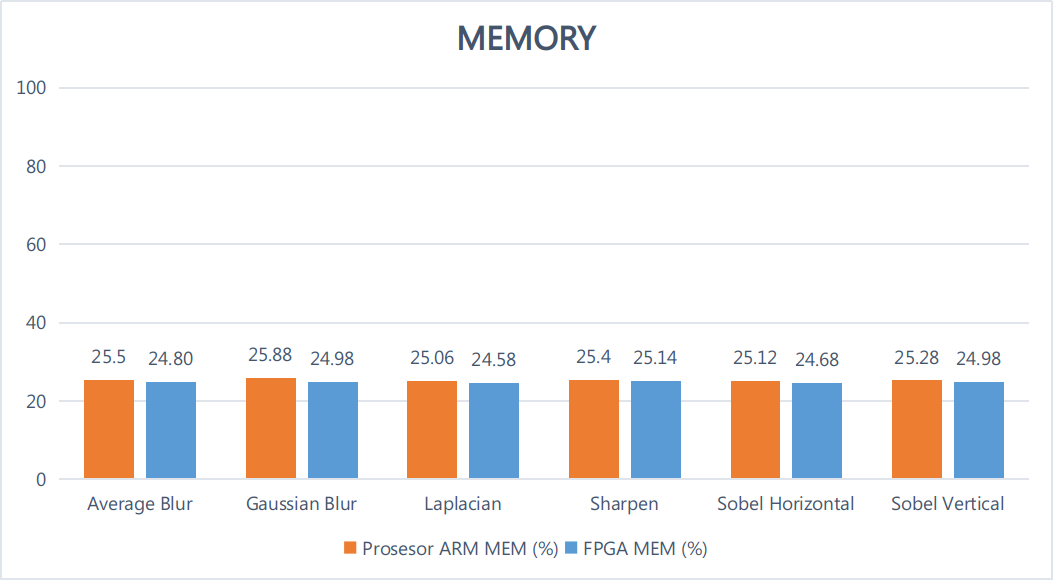
\includegraphics[width=0.81\linewidth, center]{images/chart/chart-mem.png}
    \caption{Comparison chart of Memory Utilize using ARM prosesor and FPGA.}
    \label{fig:chart-mem}
\end{figure}

% Walaupun FPGA lebih baik daripada prosesor ARM pada segi waktu komputasi dan FPS namun penggunaan \textit{memory} pada penerapan filter ini terlihat tidak jauh berbeda. Penggunaan \textit{memory} FPGA ini hanya 0,51\% lebih rendah dari penggunaan \textit{memory} dengan prosesor ARM.

Although FPGA is better than ARM processors in terms of computation time and FPS, the use of memory in the application of this filter does not look much different. This FPGA's memory usage is only 0.51\% lower than memory usage with ARM processors.

% Efisiensi penggunaan \textit{memory} yang dimiliki FPGA dibandingkan dengan prosesor ARM, dapat dihitung dengan persamaan berikut:

The efficiency of using memory owned by FPGA compared to ARM processors, can be calculated by the following equation:
\begin{equation*}
    % \label{eq:efisiensi-momory}
    \begin{split}
& = 100\% - \left( \frac{memory\ FPGA}{memory\ ARM Prosesor} \times 100\% \right) \\
& = 100\% - \left( \frac{24.86}{25.37} \times 100\% \right) \\
& = 100\% - 97.98\% \\
& = 2.02\% \\
    \end{split}
\end{equation*}
% diperoleh efisiensi penggunaan \textit{memory} FPGA dibandingkan dengan prosesor ARM adalah sebesar 2.02\%.

the efficiency of using \ textit {memory} FPGA compared to ARM processors is 2.02\%.


\subsection{Resident Memory (RES)}

% Data penggunaan \textit{resident memory} atau RES dengan prosesor ARM dan FPGA dapat dilihat pada tabel \ref{table:hasil-res} dan grafik pada gambar \ref{fig:chart-res}. Data ini menunjukkan banyaknya RES (dalam satuan \textit{kilobyte}) yang digunakan pada saat penerapan filter spasial pada video \textit{stream} dengan masing-masing kernel.

The usage of resident memory or RES with ARM processors and FPGAs can be seen in the \ref{table:hasil-res} table and the chart in the \ref{fig:chart-res} image. This data shows the number of RES (in kilobytes) used when applying the spatial filter to video stream with each kernel.

\begin{atable}
    \caption{Comparison table of resident memory (RES) using ARM prosesor and FPGA.}
    \label{table:hasil-res}
    \csvreader[
        head to column names,
        tabular=lcc,
        separator=semicolon,
        before table=\rowcolors{2}{gray!15}{gray!30},
        table head= \rowcolor{gray!50!black} 
            \color{white} Filter & 
            \color{white} Prosesor ARM (KiB) & 
            \color{white} FPGA (KiB)\\]
        {tables/hasil-res.csv}
        {
            filter=\filter, 
            arm=\arm, 
            fpga=\fpga}
        {
            \filter & 
            \arm & 
            \fpga }
\end{atable}
\begin{figure}[H]
    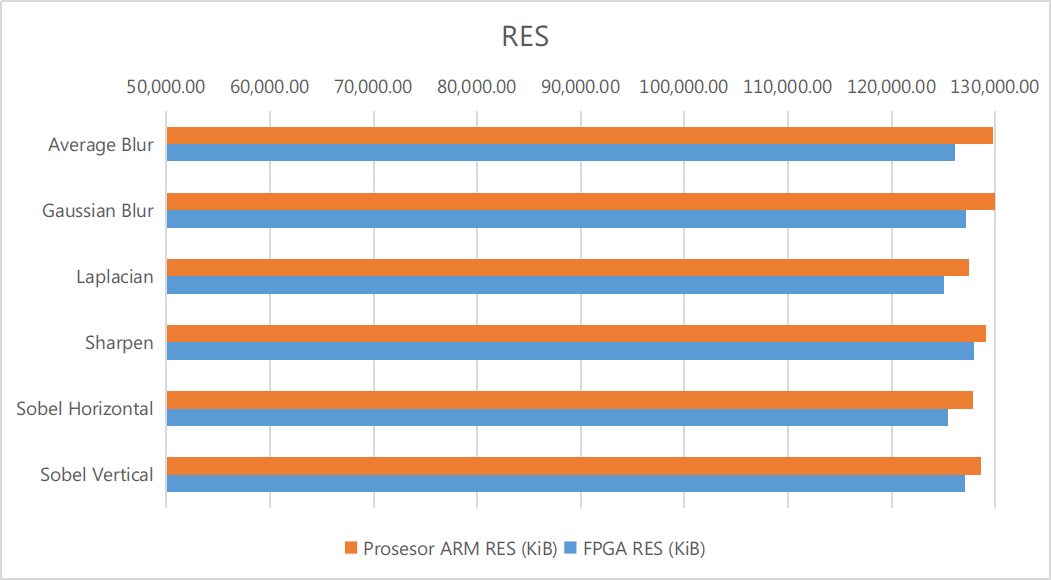
\includegraphics[width=0.81\linewidth, center]{images/chart/chart-res.png}
    \caption{Comparison chart of resident memory (RES) using ARM prosesor and FPGA.}
    \label{fig:chart-res}
\end{figure}
% Rata-rata RES yang digunakan pada prosesor ARM adalah 129108,60 KiB dan 126437,20 KiB pada FPGA. Terlihat bahwa penggunaan RES pada prosesor ARM dan FPGA juga tidak jauh berbeda. Penggunaan RES terbesar dengan prosesor ARM yaitu pada kernel \textit{gaussian blur} 131804,40 KiB, sedangkan dengan FPGA yaitu pada kernel \textit{sharpening} 127931,20 KiB.

The average RES used on ARM processors is 129108.60 KiB and 126437.20 KiB on the FPGA. It can be seen that the use of RES on ARM and FPGA processors is not much different. The biggest use of RES with ARM processors is the kernel gaussian blur 131804.40 KiB, while with FPGA is the kernel sharpening 127931.20 KiB.

% Efisiensi penggunaan \textit{resident} \textit{memory} yang dimiliki FPGA dibandingkan dengan prosesor ARM, dapat dihitung dengan persamaan berikut:

The efficient use of resident memory owned by FPGA compared to ARM processors, can be calculated by the following equation:
\begin{equation*}
    % \label{eq:efisiensi-resident-momory}
    \begin{split}
& = 100\% - \left( \frac{resident\ memory\ FPGA}{resident\ memory\ ARM Prosesor} \times 100\% \right) \\
& = 100\% - \left( \frac{126437.20}{129108.60} \times 100\% \right) \\
& = 100\% - 97.93\% \\
& = 2.07\% \\
    \end{split}
\end{equation*}
% diperoleh efisiensi penggunaan \textit{resident} \textit{memory} FPGA dibandingkan dengan prosesor ARM adalah sebesar 2.07\%.

the efficiency of the resident memory FPGA compared to ARM processors is 2.07\%.


\subsection{Shared Memory (SHR)}

% Data penggunaan \textit{shared memory} dengan prosesor ARM dan FPGA dapat dilihat pada tabel \ref{table:hasil-shr} dan grafik pada gambar \ref{fig:chart-shr}. Data ini menunjukkan banyaknya \textit{shared memory} (dalam satuan \textit{kilobyte}) yang digunakan pada saat penerapan filter spasial pada video \textit{stream} dengan masing-masing kernel.

The usage of shared memory with ARM and FPGA processors can be seen in the \ref{table:hasil-shr} and the chart in the \ref{fig:chart-shr} image. This data shows the number of shared memory (in kilobytes) used when applying the spatial filter to video stream with each kernel.

\begin{atable}
    \caption{Comparison table of shared memory (SHR) using ARM prosesor and FPGA.}
    \label{table:hasil-shr}
    \csvreader[
        head to column names,
        tabular=lcc,
        separator=semicolon,
        before table=\rowcolors{2}{gray!15}{gray!30},
        table head= \rowcolor{gray!50!black} 
            \color{white} Filter & 
            \color{white} Prosesor ARM (KiB) & 
            \color{white} FPGA (KiB)\\]
        {tables/hasil-shr.csv}
        {
            filter=\filter, 
            arm=\arm, 
            fpga=\fpga}
        {
            \filter & 
            \arm & 
            \fpga }
\end{atable}
\begin{figure}[ht]
    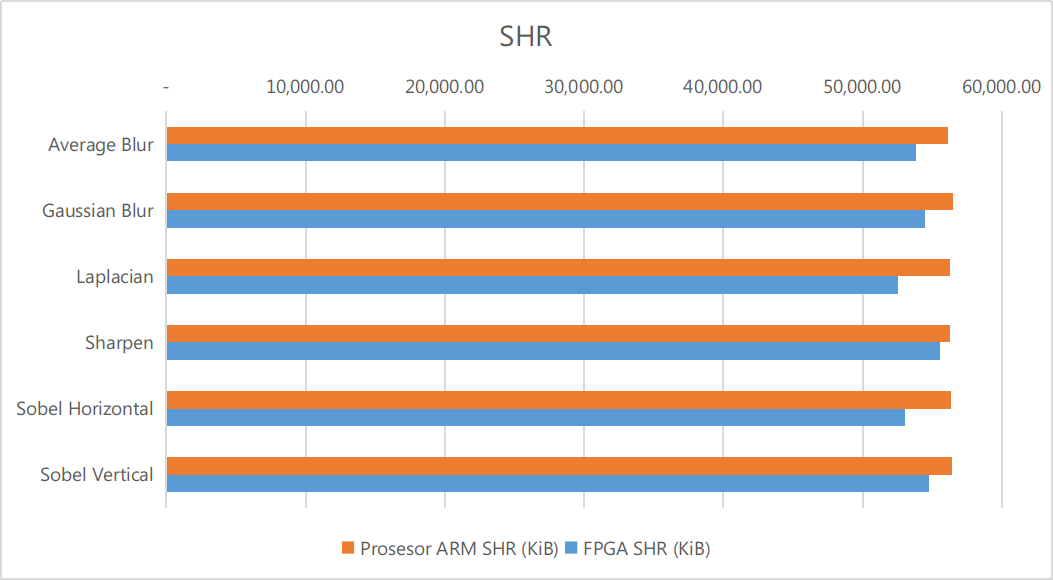
\includegraphics[width=0.81\linewidth, center]{images/chart/chart-shr.png}
    \caption{Comparison chart of shared memory (SHR) using ARM prosesor and FPGA.}
    \label{fig:chart-shr}
\end{figure}
% Rata-rata penggunaan \textit{shared memory} pada prosesor ARM adalah 56325,57 KiB dan 54030,80 KiB pada FPGA. Terlihat bahwa penggunaan \textit{shared memory} pada prosesor ARM sedikit lebih besar daripada FPGA. Penggunaan \textit{shared memory} terbesar pada prosesor ARM yaitu pada kernel \textit{gaussian blur} 56503,60 KiB dan kernel \textit{laplacian} 55528,80 KiB pada FPGA. Penggunaan \textit{shared memory} terkecil pada prosesor ARM yaitu pada kernel \textit{average blur} 56157,40 KiB dan kernel \textit{laplacian} 42568 KiB pada FPGA.

The average usage of shared memory on ARM processors is 56325.57 KiB and 54030.80 KiB on the FPGA. It can be seen that the use of shared memory on an ARM processor is slightly larger than that of an FPGA. The largest usage of shared memory on ARM processors is the 56503.60 KiB kernel gaussian blur and the 55528.80 KiB kernel laplacian on the FPGA. The smallest shared memory usage on ARM processors is the 56157.40 KiB average blur kernel and the 42568 KiB laplacian kernel on the FPGA.

% Efisiensi penggunaan \textit{shared} \textit{memory} yang dimiliki FPGA dibandingkan dengan prosesor ARM, dapat dihitung dengan persamaan berikut:

The efficiency of using shared memory owned by FPGA compared to ARM processors, can be calculated by the following equation:
\begin{equation*}
    % \label{eq:efisiensi-shared-momory}
    \begin{split}
& = 100\% - \left( \frac{shared\ memory\ FPGA}{shared\ memory\ ARM Prosesor} \times 100\% \right) \\
& = 100\% - \left( \frac{54030.80}{56325.57} \times 100\% \right) \\
& = 100\% - 95.92\% \\
& = 4.08\% \\
    \end{split}
\end{equation*}
% diperoleh efisiensi penggunaan \textit{shared} \textit{memory} FPGA dibandingkan dengan prosesor ARM adalah sebesar 4.08\%.

The efficiency of using shared memory FPGA compared to ARM processors is 4.08\%.


\subsection{Virtual Memory (VIRT)}

% Data penggunaan \textit{virtual memory} atau VIRT dapat dilihat pada tabel \ref{table:hasil-virt} dan grafik pada gambar \ref{fig:chart-virt}. Data ini menunjukkan banyaknya \textit{virtual memory} (dalam satuan \textit{kilobyte}) yang digunakan pada saat penerapan filter spasial pada video \textit{stream} dengan masing-masing kernel.

The usage of virtual memory or VIRT can be seen in the \ref{table:hasil-virt} table and the chart in the \ref{fig:chart-virt} image. This data shows the amount of virtual memory (in kilobytes) used when applying the spatial filter to video stream with each kernel.

\begin{atable}
    \caption{Comparison table of virtual memory (VIRT) using ARM prosesor and FPGA.}
    \label{table:hasil-virt}
    \csvreader[
        head to column names,
        tabular=lcc,
        separator=semicolon,
        before table=\rowcolors{2}{gray!15}{gray!30},
        table head= \rowcolor{gray!50!black} 
            \color{white} Filter & 
            \color{white} Prosesor ARM (KiB) & 
            \color{white} FPGA (KiB)\\]
        {tables/hasil-virt.csv}
        {
            filter=\filter, 
            arm=\arm, 
            fpga=\fpga}
        {
            \filter & 
            \arm & 
            \fpga }
\end{atable}
\begin{figure}[H]
    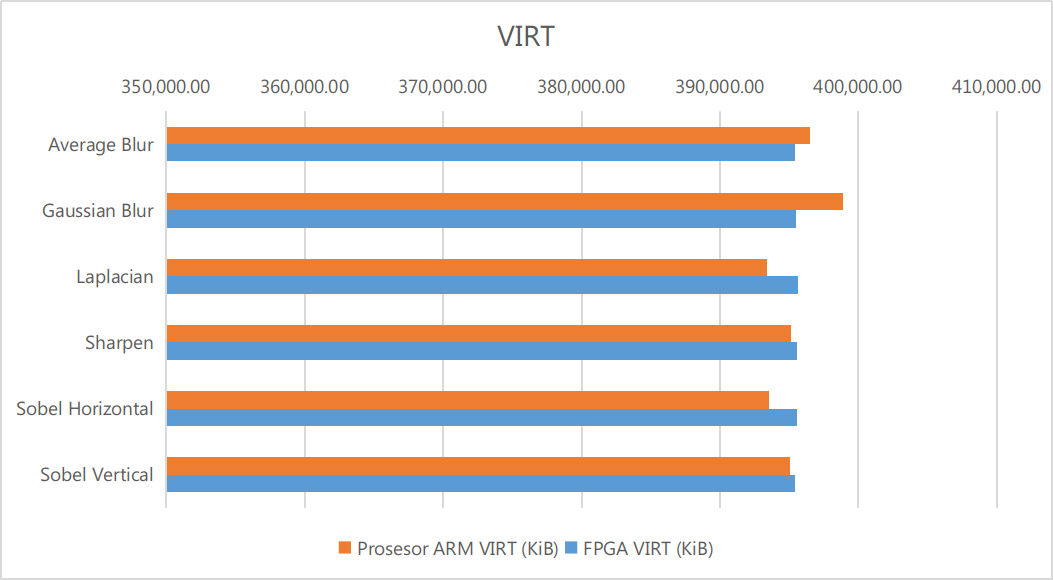
\includegraphics[width=0.81\linewidth, center]{images/chart/chart-virt.png}
    \caption{Comparison chart of virtual memory (VIRT) using ARM prosesor and FPGA.}
    \label{fig:chart-virt}
\end{figure}
% Rata-rata penggunaan VIRT pada prosesor ARM adalah 395407,64 KiB dan 395501,33 KiB pada FPGA. Rata-rata penggunaan VIRT pada FPGA sedikit lebih tinggi dari pada prosesor ARM. Penggunaan VIRT terbesar dengan prosesor ARM yaitu pada kernel \textit{gaussian blur} 398862,80 KiB dan kernel \textit{laplacian} 395638,40 KiB pada FPGA. Penggunaan VIRT terkecil dengan prosesor ARM yaitu pada kernel \textit{laplacian} 393388,00 KiB dan kernel \textit{sobel vertical} 395385,60 KiB pada FPGA.

The average VIRT usage on ARM processors is 395407.64 KiB and 395501.33 KiB on FPGAs. The average use of VIRT on FPGAs is slightly higher than on ARM processors. The biggest use of VIRT with ARM processors is the kernel gaussian blur 398862.80 KiB and kernel laplacian 395638.40 KiB on the FPGA. The smallest use of VIRT with an ARM processor is the laplacian kernel 393388.00 KiB and the kernel sobel vertical 395385.60 KiB on the FPGA.

% Efisiensi penggunaan \textit{virtual} \textit{memory} yang dimiliki prosesor ARM dibandingkan dengan FPGA, dapat dihitung dengan persamaan berikut:

The efficiency of using virtual memory owned by ARM processors compared to FPGA, can be calculated by the following equation:
\begin{equation*}
    % \label{eq:efisiensi-virtual-momory}
    \begin{split}
& = 100\% - \left( \frac{virtual\ memory\ ARM Prosessor}{virtual\ memory\ FPGA} \times 100\% \right) \\
& = 100\% - \left( \frac{395407.64}{395501.33} \times 100\% \right) \\
& = 100\% - 99.97\% \\
& = 0.03\% \\
    \end{split}
\end{equation*}

% Ini menunjukkan bahwa penggunaan \textit{virtual momory} pada prosesor ARM hanya 0.03\% lebih baik dari penggunaan \textit{virtual momory} pada FPGA.

This shows that using virtual momory on an ARM processor is only 0.03\% better than using virtual momory on an FPGA.

%------------------------------------------------
% 5. Conclusion
\section{Conclusion}

% Berdasarkan hasil penerapan filter spasial linear pada FPGA Development Board dengan menggunakan 6 kernel, peneliti dapat menarik beberapa kesimpulan sebagai berikut:

Based on the results of implementation linear spatial filters on the FPGA Development Board using 6 kernels, researchers get the following conclusions:
\begin{enumerate}[topsep=0pt,itemsep=0pt,partopsep=0pt, parsep=0pt]
    % \item Proses implementasi filter spasial linear pada video \textit{stream} dengan FPGA Development Board dilakukan dengan \textit{library} OpenCV \textit{python} dan \textit{library} xfOpenCV Xilinx. Setiap \textit{frame} dari \textit{source} video \textit{stream} direpresentasikan sebagai citra digital kemudian dilakukan filter spasial linear, selanjutnya hasil filter ini ditampilkan secara berkesinambungan sehingga tampak seperti video.

    \item The process of implementing a linear spatial filter on video stream with the FPGA Development Board is carried out with python's library OpenCV and Xilinx's library xfOpenCV. Each frame of video stream source is represented as a digital image then a linear spatial filter is applied, then the results of this filter are displayed continuously so that it looks like a video.

    % \item Waktu komputasi dengan FPGA 88.85\% lebih baik dibandingkan dengan ARM prosesor. Video hasil filter dengan ARM prosesor memperoleh rata-rata 6.95 fps sedangkan dengan FPGA rata-rata 60.37 fps. FPS dengan FPGA 88.49\% lebih baik lebih baik dibandingkan dengan ARM prosesor. Penggunaan CPU pada FPGA 14.89\% lebih baik, penggunaan \textit{memory} pada FPGA 2.02\% lebih baik, penggunaan \textit{resident memory} 2.07\% lebih baik, dan penggunaan \textit{shared memory} 4.08\% lebih baik dibandingkan dengan ARM prosesor. Sedangkan penggunaan \textit{virtual memory} pada ARM prosesor 0.03\% lebih baik dibandingkan FPGA.

    \item Compute time with FPGA 88.85\% better than ARM processor. The filtered video with the ARM processor gets an average of 6.95 fps while the FPGA average is 60.37 fps. FPS with FPGA is 88.49\% better than ARM processor. CPU loads on FPGA is 14.89\% better, usage of memory on FPGA is 2.02\% better, usage of resident memory is 2.07\% better, and usage of shared memory is 4.08\% better compared to ARM processors. Meanwhile, the use of virtual memory on ARM processors is 0.03\% better than FPGA.
\end{enumerate}